\documentclass{llncs}

\pagestyle{plain} 

\usepackage{latexsym}
\usepackage{setspace}
\usepackage{cancel}
\usepackage{listings}
\usepackage{graphicx}
\usepackage{appendix}
 \usepackage{amssymb}
\usepackage{stmaryrd}
\usepackage{amsmath}
\usepackage{leftidx}
\usepackage{mathtools}
\usepackage{paralist}
\usepackage{color}
\usepackage{mathrsfs}
\usepackage{tikz}
\usetikzlibrary{shapes}
%\usepackage{times}

\usepackage[linesnumbered,ruled]{algorithm2e}


%!TEX root = popl2018.tex

\newcommand{\set}[1]{\{ #1 \}}
\newcommand{\sequence}[2]{(#1, \ldots, #2)}
\newcommand{\couple}[2]{(#1,#2)}
\newcommand{\pair}[2]{(#1,#2)}
\newcommand{\triple}[3]{(#1,#2,#3)}
\newcommand{\quadruple}[4]{(#1,#2,#3,#4)}
\newcommand{\tuple}[2]{(#1,\ldots,#2)}
\newcommand{\Nat}{\ensuremath{\mathbb{N}}}
\newcommand{\Rat}{\ensuremath{\mathbb{Q}}}
\newcommand{\Rea}{\ensuremath{\mathbb{R}}}
\newcommand{\Zed}{\ensuremath{\mathbb{Z}}}
%\newcommand{\true}{\top}
%\newcommand{\false}{\perp}
\newcommand{\bottom}{\perp}
%% \newcommand{\powerset}[1]{{\cal P}(#1)}
\newcommand{\npowerset}[2]{{\cal P}^{#1}(#2)}
\newcommand{\finitepowerset}[1]{{\cal P}_f(#1)}
\newcommand{\level}[2]{L_{#1}(#2)}
\newcommand{\card}[1]{\mbox{card}(#1)}
\newcommand{\range}[1]{\mathtt{ran}(#1)}
\newcommand{\astring}{s}

\newcommand{\Cc}{\mathcal{C}}


\newcommand {\notof}{\ensuremath{\neg}}
\newcommand {\myand}{\ensuremath{\wedge}}
\newcommand {\myor}{\ensuremath{\vee}}
\newcommand {\mynext}{\mbox{{\sf X}}}
\newcommand {\until}{\mbox{{\sf U}}}
\newcommand {\sometimes}{\mbox{{\sf F}}}
\newcommand {\previous}{\mynext^{-1}}
\newcommand {\since}{\mbox{{\sf S}}}
\newcommand {\fminusone}{\mbox{{\sf F}}^{-1}}
\newcommand {\everywhere}[1]{\mbox{{\sf Everywhere}}(#1)}



\newcommand{\aatomic}{{\rm A}}
\newcommand{\aset}{X}
\newcommand{\asetbis}{Y}
\newcommand{\asetter}{Z}

\newcommand{\avarprop}{p}
\newcommand{\avarpropbis}{q}
\newcommand{\avarpropter}{r}
\newcommand{\varprop}{{\rm PROP}} % Set of atomic propositions (for a given logic)

% formulae

\newcommand{\aformula}{\astateformula} % a formula
\newcommand{\aformulabis}{\astateformulabis} % another formula (when at least 2 are present)
\newcommand{\aformulater}{\astateformulater} % another formula (when at least 3 are present)
\newcommand{\asetformulae}{X}
\newcommand{\subf}[1]{sub(#1)}

\newcommand{\aautomaton}{{\mathbb A}}
\newcommand{\aautomatonbis}{{\mathbb B}}

\newcommand {\length}[1] {\ensuremath{|#1|}}



% Equivalences
\newcommand{\egdef}{\stackrel{\mbox{\begin{tiny}def\end{tiny}}}{=}} % =def=
\newcommand{\eqdef}{\stackrel{\mbox{\begin{tiny}def\end{tiny}}}{=}} % =def=
\newcommand{\equivdef}{\stackrel{\mbox{\begin{tiny}def\end{tiny}}}{\equivaut}} % <=def=>
\newcommand{\equivaut}{\;\Leftrightarrow\;}

\newcommand{\ainfword}{\sigma}

\newcommand{\amap}{\mathfrak{f}}
\newcommand{\amapbis}{\mathfrak{g}}

\newcommand{\step}[1]{\xrightarrow{\!\!#1\!\!}}
\newcommand{\backstep}[1]{\xleftarrow{\!\!#1\!\!}}

\newcommand {\aedge}[1] {\ensuremath{\stackrel{#1}{\longrightarrow}}}
\newcommand {\aedgeprime}[1] {\ensuremath{\stackrel{#1}{\longrightarrow'}}}
\newcommand {\afrac}[1] {\ensuremath{\mathit{frac}(#1)}}
\newcommand {\cl}[1] {\ensuremath{\mathit{cl}(#1)}}
\newcommand {\sfc}[1] {\ensuremath{\mathit{sfc}(#1)}}
\newcommand {\dunion} {\ensuremath{\uplus}}
\newcommand {\edge} {\ensuremath{\longrightarrow}}
\newcommand {\emptyword}{\ensuremath{\epsilon}}
\newcommand {\floor}[1] {\ensuremath{\lfloor #1 \rfloor}}
\newcommand {\intersection} {\ensuremath{\cap}}
\newcommand {\union} {\ensuremath{\cup}}
\newcommand {\vals}[2] {\ensuremath{\mathit{val}_{#2}(#1)}}



\newcommand {\pspace} {\textsc{pspace}}
\newcommand {\nlogspace} {\textsc{nlogspace}}
\newcommand {\logspace} {\textsc{logspace}}
\newcommand {\expspace} {\textsc{expspace}}
\newcommand {\np} {\textsc{np}}
\newcommand {\threeexptime} {\textsc{3exptime}}
\newcommand {\polytime} {\textsc{p}}
\newcommand{\twoexpspace}{\textsc{2expspace}}
\newcommand{\threeexpspace}{\textsc{3expspace}}
\newcommand {\nexptime} {\textsc{nexptime}}



\newcommand{\aalphabet}{\Sigma}     % an alphabet, A is already used for atoms
\newcommand{\aword}{\mathfrak{u}}
\newcommand{\awordbis}{\mathfrak{v}}



\newcommand{\aassertion}{P}
\newcommand{\aassertionbis}{Q}
\newcommand{\aexpression}{e}
\newcommand{\aexpressionbis}{f}
\newcommand{\avariable}{\mathtt{x}}
\newcommand{\uniquevar}{\mathtt{u}}
\newcommand{\uniquevarbis}{\mathtt{v}}
\newcommand{\avariablebis}{\mathtt{y}}
\newcommand{\avariableter}{\mathtt{z}}
\newcommand{\nullconstant}{\mathtt{null}}
\newcommand{\nilvalue}{nil}
\newcommand{\emptyconstant}{\mathtt{emp}}
\newcommand{\infheap}{\mathtt{inf}}
\newcommand{\saturated}{\mathtt{Saturated}}

\newcommand{\astateformula}{\phi}
\newcommand{\astateformulabis}{\psi}
\newcommand{\astateformulater}{\varphi}
%%
\newcommand{\separate}{\ast}
\newcommand{\sep}{\separate}
\newcommand{\size}{\mathtt{size}}
\newcommand{\sizeeq}[1]{\mathtt{size} \ = \ #1}
\newcommand{\alloc}[1]{\mathtt{alloc}(#1)}
\newcommand{\allocb}[2]{\mathtt{alloc}^{-1}[#2](#1)}
\newcommand{\isol}[1]{\mathtt{isoloc}(#1)}
\newcommand{\icell}{\mathtt{isocell}}
\newcommand{\malloc}{\mathtt{malloc}}
\newcommand{\cons}{\mathtt{cons}}
\newcommand{\new}{\mathtt{new}}
\newcommand{\free}[1]{\mathtt{free} \ #1}
\newcommand{\maxform}[1]{\mathtt{maxForms}(#1)}
\newcommand{\locations}[1]{\mathtt{loc}(#1)}
\newcommand{\values}{\mathtt{Val}}
\newcommand{\aheap}{\mathfrak{h}}
\newcommand{\avaluation}{\mathfrak{V}}
\newcommand{\heaps}{\mathcal{H}}
\newcommand{\astore}{\mathfrak{s}}
\newcommand{\stores}{\mathcal{S}}
\newcommand{\amodel}{\mathfrak{M}}
\newcommand{\alabel}{\ell}

\newcommand{\aprogram}{\mathtt{PROG}}
\newcommand{\programs}{\mathtt{P}}
\newcommand{\ctprograms}{\programs^{ct}}
\newcommand{\aninstruction}{\mathtt{instr}}
\newcommand{\ainstruction}{\mathtt{instr}}
\newcommand{\instructions}{\mathtt{I}}
\newcommand{\aguard}{\ensuremath{g}}
\newcommand{\guards}{\ensuremath{G}}
\newcommand{\domain}[1]{\mathtt{dom}(#1)}
\newcommand{\memory}{\stores\times\heaps}
\newcommand{\skipinstruction}{\mathtt{skip}}

\newcommand{\execution}{\mathtt{comp}}
\newcommand{\aux}{\mathtt{embd}}
\newcommand{\runof}{run}
\newcommand{\anexecution}{e}


\newcommand{\aletter}{\ensuremath{a}}
\newcommand{\aletterbis}{\ensuremath{b}}
\newcommand{\alocation}{\mathfrak{l}}

\newcommand{\pointsl}[1]{\stackrel{#1}{\hookrightarrow}}
\newcommand{\ppointsl}[1]{\stackrel{#1}{\mapsto}}
\newcommand{\ourhook}[1]{\stackrel{#1}{\hookrightarrow}}
\newcommand{\ltrue}{{\sf true}}
\newcommand{\lfalse}{{\sf false}}


\newcommand{\variables}{\mathtt{FVAR}}
\newcommand{\pvariables}{\mathtt{PVAR}}
\newcommand{\secvariables}{\mathtt{SVAR}}
\newcommand{\logique}[1]{\mathtt{FO}(#1)}



\newcommand{\atranslation}{\mathfrak{t}}
\newcommand{\nbpred}[1]{\widetilde{\sharp #1}}
\newcommand{\nbpredstar}[1]{\widetilde{\sharp #1}^{\star}}
\newcommand{\isolated}{\mathtt{isol}}
\newcommand{\stdmarks}{\mathtt{envir}}
\newcommand{\relation}[1]{\mathtt{relation}_{#1}}
\newcommand{\freevar}{\mathtt{FV}}
\newcommand{\notonmark}{\mathtt{notonenv}}
\newcommand{\InVal}[1]{\mathtt{InVal}\!\left(#1\right)}
\newcommand{\NotOnEnv}[1]{\mathtt{NotOnEnv}\!\left(#1\right)}
\newcommand{\PartOfVal}[1]{\mathtt{PartOfVal}\!\left(#1\right)}
%\newcommand{\nbpreds}[3]{\sharp #1 \geq #2}
\newcommand{\defstyle}[1]{{\emph{#1}}}

\newcommand{\cut}[1]{}
\newcommand{\interval}[2]{[#1,#2]}
\newcommand{\buniquevar}{\overline{\uniquevar}}
\newcommand{\bbuniquevar}{\overline{\overline{\uniquevar}}}
\newcommand{\magicwand}{\mathop{\mbox{$\mbox{$-~$}\!\!\!\!\ast$}}}
\newcommand{\wand}{\magicwand}
\newcommand{\septraction}{\stackrel{\hsize0pt \vbox to0pt{\vss\hbox to0pt{\hss\raisebox{-6pt}{\footnotesize$\lnot$}\hss}\vss}}{\magicwand}}
%% \newcommand{\reach}{\mathtt{reach}}
\mathchardef\mhyphen="2D % hyphen while in math mode

\newcommand{\adataword}{\mathfrak{dw}}
\newcommand{\adatum}{\mathfrak{d}}

\newcommand{\collectionknives}{\mathtt{ks}}
\newcommand{\collectionknivesfork}[1]{\mathtt{ksfs}_{=#1}}
\newcommand{\collectionknivesforks}{\mathtt{ksfs}}
\newcommand{\collectionkniveslargeforks}{\mathtt{kslfs}}


\newcommand{\acounter}{\mathtt{C}}

\newcommand{\fotwo}[3]{{\mbox{FO2}_{#1,#2}(#3)}}
\newcommand{\mtrans}[1]{t\!\left(#1\right)^{\Box}}
\newcommand{\mbtrans}[2]{\mtrans{#2}_{#1}}


\newcommand{\alogic}{\mathfrak{L}}


\newcommand{\semantics}[1]{\ensuremath{[ #1 ]}}


\newcommand{\adomino}{\mathfrak{d}}
\newcommand{\atile}{\mathfrak{d}}
\newcommand{\atiling}{\mathfrak{t}}

\newcommand{\hori}{\mathtt{h}}
\newcommand{\verti}{\mathtt{v}}
\newcommand{\domi}{\mathtt{d}}

\newcommand{\cpyrel}{\mathfrak{cp}}

\newcommand{\cntcmp}{\mathfrak{C}}

\newcommand{\heapdag}{\mathfrak{G}}

\newcommand{\onmainpath}{\mathtt{mp}}

\newcommand{\tree}{\mathtt{tree}}

%\newcommand{\tile}{\mathtt{tile}}

\newcommand{\type}{\mathtt{type}}

\newcommand{\ptype}{\mathtt{ptype}}

\newcommand{\exttype}{\mathtt{exttype}}

\newcommand{\anctypes}{\mathtt{AncTypes}}

\newcommand{\destypes}{\mathtt{DesTypes}}

\newcommand{\inctypes}{\mathtt{IncTypes}}

\newcommand{\treeic}{\mathtt{treeIC}}

\newcommand{\trs}{\mathfrak{trs}}


\newcommand{\nin}{\not \in}
\newcommand{\cupplus}{\uplus}
\newcommand{\aunarypred}{\mathtt{P}}


\newcommand{\hide}[1]{}

\newcommand{\eval}[2]{\llbracket#1\rrbracket_{#2}}
\newcommand\cur{\mathsf{cur}}
\newcommand\dom{\mathsf{dom}}
\newcommand\rng{\mathsf{rng}}

\newcommand\dd{\mathbb{D}}
\newcommand\nat{\mathbb{N}}


\newcommand\cA{\mathcal{A}}
\newcommand\cB{\mathcal{B}}
\newcommand\cC{\mathcal{C}}
\newcommand\cE{\mathcal{E}}
\newcommand\cG{\mathcal{G}}
\newcommand\Ll{\mathcal{L}}
\newcommand\cM{\mathcal{M}}
\newcommand\cP{\mathcal{P}}
\newcommand\cR{\mathcal{R}}
\newcommand\cS{\mathcal{S}}
\newcommand\cT{\mathcal{T}}

\newcommand\vard{\mathfrak{d}}

\newcommand\replaceall{\mathsf{replaceAll}}
\newcommand\indexof{\mathsf{IndexOf}}


\newcommand\strline{\mathsf{SL}}

\newcommand\pstrline{\mathsf{SL_{pure}}}

\newcommand\search{\mathsf{search}}

\newcommand\verify{\mathsf{verify}}

\newcommand\searchleft{\mathsf{searchLeft}}

\newcommand\searchlong{\mathsf{searchLong}}


\newcommand\pref{\mathsf{Pref}}

\newcommand\wprof{\mathsf{WP}}

\newcommand\vars{\mathsf{Vars}}

\newcommand\dep{\mathsf{Dep}}
\newcommand\ptn{\mathsf{Ptn}}

\newcommand\src{\mathsf{src}}
\newcommand\strtorep{\mathsf{strToRep}}

\newcommand\rpleft{\mathsf{l}}
\newcommand\rpright{\mathsf{r}}


\newcommand\srcnd{\mathsf{srcND}}

\newcommand\ctxt{\mathsf{ctxt}}


\newcommand\ctxts{\mathsf{Ctxts}}

\newcommand\sprt{\mathsf{sprt}}

\newcommand\val{\mathsf{val}}

\newcommand\srclen{\mathsf{srcLen}}

\newcommand\rpleftlen{\mathsf{lLen}}


\newcommand\dfs{\mathsf{DFS}}

\newcommand\repr{\mathsf{rep}}

\newcommand\red{\mathsf{red}}

\newcommand\gfun{\mathcal{F}}


\newcommand{\leftmost}{{\sf leftmost}}
\newcommand{\longest}{{\sf longest}}

\newcommand{\arbidx}{{\sf Idx_{arb}}}
\newcommand{\dmdidx}{{\sf Idx_{dmd}}}
\newcommand{\lftlen}{{\sf Len_{lft}}}

%\newtheorem{remark}[theorem]{Remark}



\newcommand{\yan}[1]{\color{green} {YA: #1 :AY} \color{black}}
\newcommand{\zhilin}[1]{\color{cyan} {ZL: #1 :LZ} \color{black}}
\newcommand{\tl}[1]{\color{blue} {TL: #1 :LT} \color{black}}

\title{Decision Procedures for String Constraints \\
with ReplaceAll function}
\titlerunning{}
\author{}
\institute{}


\author{Taolue Chen, Yan Chen, Matthew Hague, Anthony W. Lin, Zhilin Wu}
\begin{document}

\maketitle


\begin{abstract}
Our goal in this note is to investigate whether we can find a fragment of string constraints which, on the one hand, includes the complex string manipulating functions $\replaceall(x, u, y)$ (where $u$ is a string, and $x,y$ are string variables), and on the other hand, enjoys a sound and complete decision procedure.
\end{abstract}

\newcommand{\concat} {\circ}

\newcommand{\replace} {{\sf replace}}

\newcommand{\str} {{\sf Str}}

\newcommand{\intnum} {{\sf Int}}

\newcommand{\regexp} {{\sf RegExp}}

\newcommand{\strarr} {{\sf StringArray}}

\newcommand{\dtypes} {{\sf DataTypes}}

\newcommand{\anarr} {{\mathbb{A}}}

\section{Introduction}

\cite{LB16,TCJ16,YABI14}

\section{Killer examples}

%https://github.com/kimmobrunfeldt/progressbar.js/blob/master/src/utils.js

\begin{verbatim}

// Renders templates with given variables. Variables must be surrounded with
// braces without any spaces, e.g. {variable}
// All instances of variable placeholders will be replaced with given content
// Example:
// render('Hello, {message}!', {message: 'world'})
function render(template, vars) {
    var rendered = template;

    for (var key in vars) {
        if (vars.hasOwnProperty(key)) {
            var val = vars[key];
            var regExpString = '\\{' + key + '\\}';
            var regExp = new RegExp(regExpString, 'g');

            rendered = rendered.replace(regExp, val);
        }
    }

    return rendered;
}
\end{verbatim}

\section{Preliminaries}

For $k \in \Nat$, let $[k] = \{1,\dots, k\}$.

For a vector $\vec{x}=(x_1,\dots, x_n)$, let $|\vec{x}|$ denote $n$ and for each $i \in [n]$, let $\vec{x}(i)$ denote $x_i$. For a vector $\vec{x} = (x_1, \dots, x_n)$, let $\red(\vec{x})$ denote $(x_{i_1},\dots, x_{i_m})$ such that for each $j \in [m]$, $x_{i_j}$ is different from all $x_1, \dots, x_{i_j-1}$.

An alphabet $\Sigma$ is fixed.

We consider the following data types: String data type $\str$, Integer data type $\intnum$, and Array of strings $\str [\ ]$.


We assume a countably set of variables, of data types form $\dtypes$. We will use $x, y, z, \dots$ to denote the variables of data type $\str$, and $n, n', \dots$ to denote the variables of type $\intnum$. In addition, we use $X, Y, Z, \dots$ to denote the variables of data type $\str[\ ]$.
We use $u, v, w, \dots$ to denote the constant strings, and $c, c',\dots$ to denote the constant integers.


For a string $u \in \Sigma^+$, let $|u|$ denote the length of $u$, in addition, for $i \in [|u|]$, let $u[i]$ the $i$-th letter of $u$.

\begin{definition}[Regular expressions $\regexp$]
\[e \eqdef a \mid e + e \mid e \concat e \mid e^\ast, \mbox{ where } a \in \Sigma. \]
We also use the abbreviations $\Sigma \equiv \cup_{a \in \Sigma}\ a$ and $\Sigma^\ast \equiv (\cup_{a \in \Sigma}\ a)^\ast$.
\end{definition}

%%%%%%%%%%%%%%%%%%%%%%%%%%%%%%%%%%%%%%%%%%%%
\hide{
A regular expression $e$ is said to be \emph{bounded} if $e$ is defined by the rules, $e \eqdef a \mid u^\ast \mid e \concat e$, where $u$ is a constant string. For instance, $a (bc)^\ast$ is bounded, while $(ab^\ast)^\ast$ is not. A regular expression $e$ is a union of bounded regular expressions if $e = e_1 + \dots + e_k$ such that each $e_i$ is a bounded regular expression. We use UBR to abbreviate the set of regular expressions which are a union of bounded regular expressions.
}
%%%%%%%%%%%%%%%%%%%%%%%%%%%%%%%%%%%%%%%%%%%%

A nondeterministic finite automata (NFA) $\cA$ on $\Sigma$ is a tuple $(Q, \delta, q_0, F)$, where $Q$ is a finite set of states, $q_0 \in Q$ is the initial state, $F \subseteq Q$ is the set of final states, and $\delta \subseteq Q \times \Sigma \times Q$ is the transition relation. An NFA $\cA$ is deterministic if for each $(q, \sigma) \in Q \times \Sigma$, there is at most one $q' \in Q$ such that $(q, a, q') \in \delta$. An NFA $\cA$ is complete if for each $(q, \sigma) \in Q \times \Sigma$, there is at least one $q' \in Q$ such that $(q, a, q') \in \delta$. We assume that all NFA considered in this paper are complete. For a string $w = \sigma_1 \dots \sigma_n$, a run of $\cA$ on $w$ is a sequence $q_0 \dots q_n$ such that for each $i \in [n]$, $(q_{i-1}, \sigma_i, q_i) \in \delta$. A run $q_0 \dots q_n$ is accepting if $q_n \in F$. A string $w$ is accepted by $\cA$ if there is an accepting run of $\cA$ on $w$. An NFA $\cA$ is \emph{unambiguous} if for each word $w$, there is \emph{at most one accepting} run of $\cA$ on $w$.
We also use the notation $q_1 \xrightarrow[\cA]{w} q_{n+1}$ to denote the fact that there are $q_2,\dots, q_n \in Q$ such that for each $i \in [n]$, $(q_i, \sigma_i, q_{i+1}) \in \delta$.  


\section{Semantics of the function $\replaceall$}

The semantics of $\replaceall(x, u, y)$ is defined inductively as follows: let $u = u_1 \dots u_k$ (where $k \ge 1$),
\begin{itemize}
\item if $x \not \in \Sigma^\ast u \Sigma^\ast$, then $\replaceall(x, u, y) = x$, 
%
\item otherwise, let $x = x' u z$ such that $x' u_1 \dots u_{k-1} \not \in \Sigma^\ast u \Sigma^\ast$, then $\replaceall(x, u, y) = x' v \cdot \replaceall(z, u, y)$.
\end{itemize}
For instance, $\replaceall(aaaaa, aaa, y) = yaa$, and $\replaceall("Jeve", e, a) = Java$.

\tl{Anthony mentioned that there might be alternatives, for instance,  $\replaceall$ can be made nondeterministic ($\replaceall(aaaaa, aaa, y) = \{yaa, aya, aay\}$). This MIGHT be considered as well.}

%%%%%%%%%%%%%%%%%%%%%%%%%%%%%%%%%%%%%%%%%%%%%%
%%%%%%%%%%%%%%%%%%%%%%%%%%%%%%%%%%%%%%%%%%%%%%
\hide{
\smallskip

\noindent The semantics of $split(x, u)$ is defined inductively as follows:
\begin{itemize}
\item if $x \not \in \Sigma^\ast u \Sigma^\ast$, then $split(x,u) = x$, 
%
\item otherwise, let $x = y u z$ such that $y \not \in \Sigma^\ast u \Sigma^\ast$, then $split(x, u) = concat([y], split(z, u))$, where $[y]$ is the array comprising one element $y$ and $concat$ operation concatenates two arrays into one.  
\end{itemize} 

For instance, $split("Java", a) = [``J", ``v", ``"]$.

\smallskip

\noindent The semantics of $join(X)$ is defined inductively as follows: 
\begin{itemize}
\item if $X$ is the empty array, then $join(X) = ``''$,  
\item otherwise, let $X= concat([x], Y)$, then $join(X) = x\ \cdot\ ``," \ \cdot\ join(Y)$.
\end{itemize}
For instance, $join([``Tom", ``John", ``Henry"]) =``Tom,John,Henry"$.
}
%%%%%%%%%%%%%%%%%%%%%%%%%%%%%%%%%%%%%%%%%%%%%%
%%%%%%%%%%%%%%%%%%%%%%%%%%%%%%%%%%%%%%%%%%%%%%

\section{Straight-line string constraint with $\replaceall$  function}


\begin{definition}[Relational and regular constraints with $\replaceall$ function]
Relational constraints and regular constraints are defined by the following rules,
\[
\begin{array}{r c l cr}
s &\eqdef & x \mid u & \ \ & \mbox{(string terms)}\\
%t &\eqdef & s \mid e & \ \ & \mbox{(terms)}\\
\varphi &\eqdef & y = s_1 \concat \dots \concat s_n (n \in \Nat) \mid  x = \replaceall(y, u, s) \mid \varphi \wedge \varphi & \ \ & \mbox{(relational constraints)}\\
\psi & \eqdef & x \in e \mid \psi \wedge \psi \mid \psi \vee \psi \mid \neg \psi   & \ \ & \mbox{(regular constraints)} \\
\end{array}
\]
where $u \in \Sigma^\ast$ and $e$ is a regular expression. 
%A regular constraint $\psi$ is a UBR constraint if for each atom $x \in e$ occurring in $\psi$, $e$ is in UBR.
\end{definition}
For a formula $\varphi$, let $\vars(\varphi)$ denote the set of variables occurring in $\varphi$. Similarly for $\vars(\psi)$.

\tl{can the regular constraints be simplified to just a conjunction of $x\in e$?}

Given a relational constraint $\varphi$, a variable $x$ (of type $\str$) is called a \emph{source variable} of $\varphi$ if $\varphi$ \emph{does not} contain a conjunct of the form $x = s_1 \concat \dots \concat s_n$ or $x = \replaceall(\dots)$.

\tl{note that here the pattern $u$ is a constant, but we may also introduce a variable here, though its decidability is not clear.} 

%%%%%%%%%%%%%%%%%%%%%%%%%%%%%%%%%%%%%%%%%%
\hide{
\begin{definition}[Dependency graph]
Let $\varphi$ be a relational constraint with $\replaceall$ function. Then the dependency graph of $\varphi$, denoted by $\cG_\varphi = (\vars(\varphi), E_\varphi)$, where $E_\varphi$ comprises the following edges,
\begin{itemize}
\item for each atomic formula $y= s_1 \concat \dots \concat s_n$ and each $i \in [n]$ such that $s_i$ is a variable, $(s_i, y) \in E_\varphi$,
\item for each atomic formula $x = \replaceall(y, u, s)$, $(y, x) \in E_\varphi$, in addition, if $s$ is a variable, then $(s, x) \in E_\varphi$, $(s, y) \in E_\varphi$, 
\end{itemize}
\end{definition}
}
%%%%%%%%%%%%%%%%%%%%%%%%%%%%%%%%%%%%%%%%%%%

\begin{definition}[Straight-line relational constraints with $\replaceall$ function]
A relational constraint $ \varphi$ with $\replaceall$ function is straight-line, if $\varphi \eqdef \bigwedge \limits_{1 \le i \le m} x_i = P_i$ such that
\begin{itemize}
\item $x_1,\dots, x_m$ are mutually distinct,
\item for each $i \in [m]$, all the variables in $P_i$ are either source variables, or variables from $\{x_1,\dots, x_{i-1}\}$,
\end{itemize}
\end{definition}
Intuitively, in a straight-line relational constraint, the dependency graph of the string variables is acyclic.


\begin{definition}[Straight-line string constraints with $\replaceall$ function]
A straight-line string constraint $C$ with $\replaceall$ function (denoted by $\strline[\replaceall]$)  is defined as $ \varphi \wedge \psi$,  where 
\begin{itemize}
\item $\varphi$ is a straight-line relational constraint,  and
%
\item $\psi$ is a regular constraint.
%
\end{itemize}
%Let us use $\Cc$ to denote the set of straight-line string constraints with $\replaceall$ function.
An $\strline[\replaceall]$ constraint $\varphi \wedge \psi$ is called \emph{pure} if the concatenation symbol $\concat$ does not occur in $\varphi$. Let us use $\pstrline[\replaceall]$ to denote the set of pure $\strline[\replaceall]$ constraints.
\end{definition}
%An SL[$replace$] constraint $\Cc=\varphi \wedge \psi$ is \emph{recursion-free} if $\varphi$ is.


\noindent {\bf Satisfiability problem}: Given an $\strline[\replaceall]$ constraint $C$, decide whether $C$ is satisfiable.

The questions we plan to consider is summarized in the following table. Note that for $x=\replaceall (y,u,z)$, $y$ is referred to as a \emph{pattern} and $z$ is referred to as a \emph{replacement}.

\[
\begin{tabular}{c|c|c|c}
                             pattern (y)  &   replacement (z)        &   pure (without concatenation) &  full (with concatenation) \\
                              \hline
                              constant  &   constant                       & \cite{LB16}    &  \cite{LB16}   \\
 \hline
                              constant  &   variable                       &  Section \ref{sec:replaceallpure}       &    \\
 \hline
                              variable  &   constant                       &         &    \\
\hline
                              variable  &   variable                       &        &    \\
\end{tabular}
\]


\section{A decision procedure for $\pstrline[\replaceall]$} \label{sec:replaceallpure}



\subsection{The single-letter case}

We start with the single-letter special case, that is, given an $\pstrline[\replaceall]$ formula $C$, it holds that every term of the form $\replaceall(z, u, z')$ in $C$ satisfies that $u$ is a single letter.

We first introduce a concept of dependency graphs.

\begin{definition}[Dependency graph]
Let $C= \varphi \wedge \psi$ be an $\pstrline[\replaceall]$ formula such that $\vars(\varphi) = \{x_1,\dots, x_m, y_1, \dots, y_n\}$, where $y_1,\dots, y_n$ are the source variables. Define the \emph{dependency graph} of $C$ as $G_C= (\vars(\varphi), E_C)$, such that for each $i \in [m]$, if $x_i = \replaceall(z, a_i, z')$, then $(x_i, (\rpleft, a_i), z) \in E_C$ and $(x_i, (\rpright, a_i), z') \in E_C$. A final (resp. initial) vertex in $G_C$ is a vertex in $G_C$ without successors (resp. predecessors). The edges labeled by $(\rpleft,a_i)$ and $(\rpright, a_i)$ are called the $\rpleft$-edges and $\rpright$-edges respectively. 
%The $\rpleft$-length of a path $\pi$, denoted by $\rpleftlen(\pi)$, is the number of $\rpleft$-edges on $\pi$. A path of $G_C$ is a sequence $z_1 \ell_1 z_2 \dots \ell_{k-1} z_k$ such that for each $i \in [k-1]$, $(z_i, \ell_i, z_{i+1}) \in E_C$. A path is initial (resp. final) if the path starts from an initial vertex (resp. stops at a final vertex).
% e the $\src$-nesting-depth of $z$ in $G_C$, denoted by $\srcnd_{G_C}(z)$,  as the maximum number of $\src$-edges in paths from source variables to $z$.
\end{definition}
Note that $G_C$ is a DAG where the out-degree of each vertex is two or zero. 


For each tuple of strings $\vec{v}=(v_1,\dots, v_n)$, if for each $j \in [n]$, $y_j$ is assigned with the string $v_j$, then for each vertex $z$ in $G_C$, the value of $z$, denoted by $\val_{\vec{v}}(z)$, is determined by the values of those source variables $y_j$ that are reachable from $z$, and can be computed in a bottom-up way. 

\smallskip


We will use the following running example to illustrate the decision procedure.
%\begin{example}
Consider the $\pstrline[\replaceall]$ formula $C=\varphi \wedge \psi$, whose dependency graph of $\varphi$ is illustrated in Fig.~\ref{fig-one-letter} and the regular constraint $\psi = \bigwedge \limits_{i \in [4]} x_i \in e_i \wedge \bigwedge \limits_{j \in [5]} y_j \in e'_j$. For $i \in [4]$ and $j \in [5]$, let us use $\cA_{x_i}$ and $\cA_{y_j}$ to denote the DFA corresponding to $e_i$ and $e'_j$ respectively.
\begin{figure}[htbp]
\begin{center}
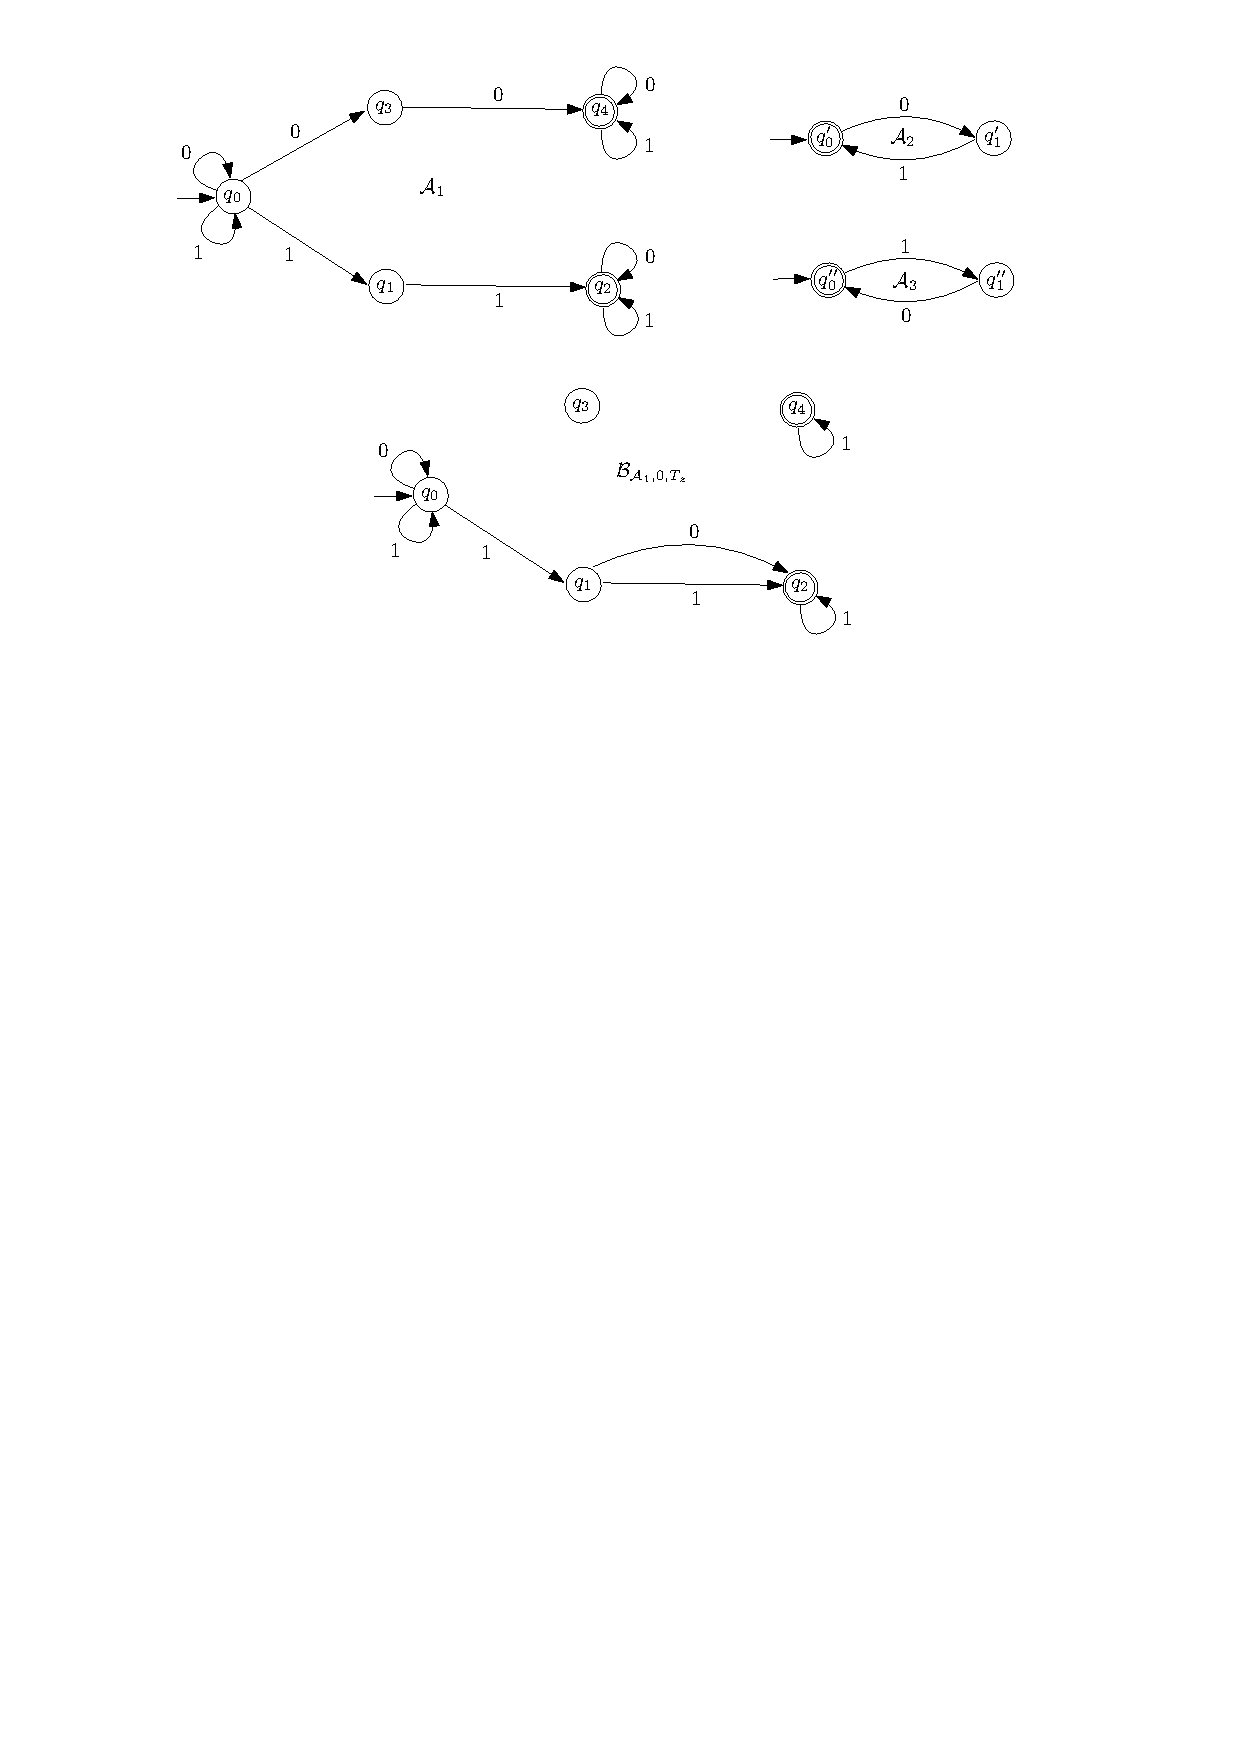
\includegraphics[scale=0.9]{single-letter-example.pdf}
\end{center}
\caption{The running example for the single-letter case}\label{fig-one-letter}
\end{figure}
%\end{example}
%



We will construct an NFA $\cA_C$ and reduce the satisfiability of $C=\varphi \wedge \psi$ to the nonemptiness of $\cA_C$. The inputs of $\cA_C$ are of the form $\triangleright \# v_1 \# \dots \# v_5\triangleleft$, where $v_1,\dots, v_5$ represent an assignment of the variables $y_1,\dots, y_5$. Intuitively, 
\begin{itemize}
\item 
 $\cA_C$ checks whether for each $j \in [5]$, $v_j$ is accepted by $\cA_{y_j}$, 
\item 
in addition, let $\vec{v} = (v_1,\dots, v_5)$, then $\cA_C$ reads $\triangleright \# v_1 \# \dots \# v_5\triangleleft$, from left to right, and checks whether $\val_{\vec{v}}(x_i)$ is accepted by $\cA_{x_i}$, for each $i \in [4]$.
\end{itemize}

In the following, we will use the running example to give a more specific description of $\cA_C$. Let us introduce some additional notations.

\begin{definition}[$\cA$-context $\ctxt$ and $\red_\ctxt$]
Suppose $\cA=(Q, \delta, q_0, F)$ is a DFA. Then an $\cA$-\emph{context} $\ctxt$  is a sequence $(a_1,f_1) \dots  (a_r, f_r)$ such that for each $i \in [r]$, $a_i \in \Sigma$ and $f_i$ is a function from $Q$ to $Q$. 
For an $\cA$-context $\ctxt$, define the reduction of $\ctxt$, denoted by $\red_\ctxt$, as follows: $\red_\ctxt = (a_{i_1},f_{i_1})  \dots  (a_{i_s}, f_{i_s})$ such that for each $j \in [s]$, $a_{i_j} \not \in \{a_1,\dots, a_{i_j-1}\}$. 
\end{definition}
Intuitively, a reduction of $\ctxt$ is obtained by keeping the first occurrence of the letters and removing the other copies.

\begin{definition}[$\cB_{\cA, \ctxt}$]
Suppose $\cA=(Q, \delta, q_0, F)$ is a DFA and $\ctxt$ is an $\cA$-context with $\red_\ctxt= (a_1,f_1) \dots  (a_r, f_r)$. We define a DFA $\cB_{\cA, \ctxt}$ as $(Q, \delta', q_0, F)$, where $\delta'$ comprises 1) all the tuples $(q, a', q') \in \delta$ with $a' \not \in \{a_1,\dots, a_r\}$, and 2) all the tuples $(q, a_i, f_i(q))$ such that $q \in Q$ and $i \in [r]$.
\end{definition}
Intuitively, over an input $w$, the DFA $\cB_{\cA, \ctxt}$ simulates the run of $\cA$ on $w$, with the following adaptation: let $\red_\ctxt= (a_1,f_1) \dots (a_r, f_r)$, then upon reading an occurrence of $a_i$, let $q$ be the current state, then after reading $a_i$, the state is changed to $f_i(q)$.

%\begin{definition}[Representatives of variables]
%For a variable $z \in \vars(\varphi)$,
%we define the representative of $z$, denoted by $\repr(z)$, as follows: If $z = y_j$ for some $j$, then $\repr(z) = y_j$, otherwise, let $\repr(z)$ be the unique source variable $y_j$ such that  there is a path from $x_i$ to $y_j$ where all edges are $\rpleft$-edges (The uniqueness of $y_j$ follows from the straight-line constraint). 
%\end{definition}

\begin{definition}[representative path]
For a non-source variable $x_i \in \vars(\varphi)$, we define the representative path of $x_i$ as the unique path from $x_i$ to some source variable $y_j$ where all the edges are $\rpleft$-edges.  For a source variable $y_j$, define the representative path of $y_j$ be the empty path.
%Note that for each non-source variable $x_i$, there is a unique source variable $y_j$ representing $x_i$. Let $\repr(x_i)$ denote this unique source variable $y_j$.
\end{definition}


We are ready to describe more details of the run of $\cA_C$ on $\triangleright \# v_1 \# \dots \# v_5\triangleleft$.

At first, for each path $\pi$ from a non-source variable $x_i$ to a source variable $y_j$,
 %such that the label sequence of $\pi$ belongs to $\rpright^\ast \rpleft^\ast$, 
 $\cA_C$ guesses a function $f_{\pi}$ on the state space of $\cA_{x_i}$, satisfying the following constraint: for each non-source variable $x_i$, let $\pi$ be the representative path of $x_i$, then $f_{\pi}(q_{0,x_i}) \in F_{x_i}$, where $q_{0, x_i}$ and $F_{x_i}$ are the initial state and the set of final states of $\cA_{x_i}$ respectively. 
% 
%Notice that for a given pair of variables $(x_i, y_j)$, let $N$ be the maximum length (number of edges) of the paths from $x_i$ to $y_j$, then there are at most $N+1$ distinct paths from $x_i$ to $y_j$ whose label sequences belong to $\rpright^\ast \rpleft^\ast$. Therefore, \emph{only polynomially many functions are guessed}.
%
%
Since $G_C$ is a tree, for simplicity, given a pair of distinct variables $z,z'$ such that $z'$ is reachable from $z$, we will use $\pi_{z,z'}$ to denote the unique path from $z$ to $z'$.  Let $\gfun$ denote the set of guessed functions.


Then $\cA_C$ verifies that the guessed functions satisfy some desired properties, when reading $\triangleright \# v_1 \# \dots \# v_5\triangleleft$.


For a path $\pi$, we define the context of $\pi$, denoted by $\ctxt_\pi$, inductively as follows: 
\begin{itemize}
\item if $\pi$ is an empty path, then $\ctxt_\pi$ is the empty vector,
% 
\item otherwise, let the last edge of $\pi$ be from $z$ to $z'$ and $\pi'$ be the path obtained from $\pi$ by removing the last edge, then 
\begin{itemize}
\item if the last edge of $\pi$ is labeled by $(\rpright, a)$, then $\ctxt_\pi = \ctxt_{\pi'}$, 
%
\item if the last edge of $\pi$ is labeled by $(\rpleft, a)$,  let $z''$ be the destination vertex of the $\rpright$-edge out of $z$ and $\pi''$ denote the path obtained by concatenating $\pi'$, the $\rpright$-edge from $z$ to $z''$, and the representative path pf $z''$, then $\ctxt_\pi = (a, f_{\pi''}) \ctxt_{\pi'}$. 
%
\end{itemize}
\end{itemize}

For instance,  
$$
\begin{array}{l c l}
\ctxt_{\pi_{x_1, y_1}} &= & (a_3, f_{\pi_{x_1, y_2}}) \ctxt_{\pi_{x_1,x_3}} = (a_3, f_{\pi_{x_1, y_2}}) (a_2, f_{\pi_{x_1, y_3}}) \ctxt_{\pi_{x_1, x_2}}  \\
& = & (a_3, f_{\pi_{x_1, y_2}}) (a_2, f_{\pi_{x_1, y_3}}) (a_1, f_{\pi_{x_1, y_4}}).
\end{array}
$$

When reading $v_1$, $\cA_C$ does the following,
\begin{itemize}
\item $\cA_C$ runs $\cA_{y_1}$ on $v_1$ to check that $v_1$ is accepted by $\cA_{y_1}$,
%
\item $\cA_C$ runs $\cB_{\cA_{x_3}, \ctxt_{\pi_{x_3,y_1}}}$ on $v_1$ to compute a function $f'_{\pi_{x_3,y_1}}$ on the state space of $\cA_{x_3}$ and checks $f'_{\pi_{x_3, y_1}} = f_{\pi_{x_3, y_1}}$,
%
\item  $\cA_C$ runs $\cB_{\cA_{x_2}, \ctxt_{\pi_{x_2,y_1}}}$ on $v_1$ to compute a function $f'_{\pi_{x_2,y_1}}$ on the state space of $\cA_{x_2}$ and checks $f'_{\pi_{x_2, y_1}} = f_{\pi_{x_2, y_1}}$, 

% if $a_2 = a_3$, then $\cA_C$ runs $\cB_{\cA_{x_2}, a_3, f_{x_2, y_2}}$ on $v_1$ to compute a function $f'_{x_2,y_1}$  on the state space of $\cA_{x_2}$ and checks $f'_{x_2, y_1} = f_{x_2, y_1}$, otherwise, $\cA_C$ runs $\cB_{\cB_{\cA_{x_2}, a_3, f_{x_2, y_2}}, a_2, f_{x_2, y_3}}$ on $v_1$ to compute $f'_{x_2,y_1}$ and checks $f'_{x_2, y_1} = f_{x_2, y_1}$,
%
\item $\cA_C$ runs $\cB_{\cA_{x_1}, \ctxt_{\pi_{x_1,y_1}}}$ on $v_1$ to compute a function $f'_{\pi_{x_1,y_1}}$  on the state space of $\cA_{x_1}$ and checks $f'_{\pi_{x_1, y_1}} = f_{\pi_{x_1, y_1}}$.
\end{itemize}
We can also think the run of $\cA_C$ on $v_1$ as the run of $\cB_{y_1, \gfun}$ on $v_1$, where  $\cB_{y_1, \gfun}$ is the product automaton of $\cA_{y_1}$, $\cB_{\cA_{x_3}, \ctxt_{\pi_{x_3,y_1}}}$, $\cB_{\cA_{x_2}, \ctxt_{\pi_{x_2,y_1}}}$, and $\cB_{\cA_{x_1}, \ctxt_{\pi_{x_1,y_1}}}$. 

When reading $v_2$, $\cA_C$ does the following,
\begin{itemize}
\item $\cA_C$ runs $\cA_{y_2}$ on $v_2$ to check that $v_2$ is accepted by $\cA_{y_2}$,
%
\item $\cA_C$ runs $ \cA_{x_3}$ on $v_2$ to compute a function $f'_{\pi_{x_3,y_2}}$ on the state space of $\cA_{x_3}$ and checks $f'_{\pi_{x_3,y_2}} = f_{\pi_{x_3, y_2}}$,
%
\item  $\cA_C$ runs $\cB_{\cA_{x_2}, \ctxt_{\pi_{x_2,y_2}}}$ on $v_2$ to compute a function $f'_{\pi_{x_2,y_2}}$ on the state space of $\cA_{x_2}$ and checks $f'_{\pi_{x_2,y_2}} = f_{\pi_{x_2, y_2}}$, 

% if $a_2 = a_3$, then $\cA_C$ runs $\cB_{\cA_{x_2}, a_3, f_{x_2, y_2}}$ on $v_1$ to compute a function $f'_{x_2,y_1}$  on the state space of $\cA_{x_2}$ and checks $f'_{x_2, y_1} = f_{x_2, y_1}$, otherwise, $\cA_C$ runs $\cB_{\cB_{\cA_{x_2}, a_3, f_{x_2, y_2}}, a_2, f_{x_2, y_3}}$ on $v_1$ to compute $f'_{x_2,y_1}$ and checks $f'_{x_2, y_1} = f_{x_2, y_1}$,
%
\item $\cA_C$ runs $\cB_{\cA_{x_1}, \ctxt_{\pi_{x_1,y_2}}}$ on $v_2$ to compute a function $f'_{\pi_{x_1,y_2}}$  on the state space of $\cA_{x_1}$ and checks $f'_{\pi_{x_1, y_2}} = f_{\pi_{x_1, y_2}}$.
\end{itemize}
We can also think the run of $\cA_C$ on $v_2$ as the run of $\cB_{y_2, \gfun}$ on $v_2$, where  $\cB_{y_2, \gfun}$ is the product automaton of $\cA_{y_2}$, $ \cA_{x_3}$, $\cB_{\cA_{x_2}, \ctxt_{\pi_{x_2,y_2}}}$, and $\cB_{\cA_{x_1}, \ctxt_{\pi_{x_1,y_2}}}$. 


When reading $v_3$, $\cA_C$ does the following,
\begin{itemize}
\item $\cA_C$ runs $\cA_{y_3}$ on $v_3$ to check that $v_3$ is accepted by $\cA_{y_3}$,
%
\item  $\cA_C$ runs $\cA_{x_2}$ on $v_3$ to compute a function $f'_{\pi_{x_2,y_3}}$ on the state space of $\cA_{x_2}$ and checks $f'_{\pi_{x_2,y_3}} = f_{\pi_{x_2, y_3}}$, 

% if $a_2 = a_3$, then $\cA_C$ runs $\cB_{\cA_{x_2}, a_3, f_{x_2, y_2}}$ on $v_1$ to compute a function $f'_{x_2,y_1}$  on the state space of $\cA_{x_2}$ and checks $f'_{x_2, y_1} = f_{x_2, y_1}$, otherwise, $\cA_C$ runs $\cB_{\cB_{\cA_{x_2}, a_3, f_{x_2, y_2}}, a_2, f_{x_2, y_3}}$ on $v_1$ to compute $f'_{x_2,y_1}$ and checks $f'_{x_2, y_1} = f_{x_2, y_1}$,
%
\item $\cA_C$ runs $\cB_{\cA_{x_1}, \ctxt_{\pi_{x_1,y_3}}}$ on $v_3$ to compute a function $f'_{\pi_{x_1,y_3}}$  on the state space of $\cA_{x_1}$ and checks $f'_{\pi_{x_1, y_3}} = f_{\pi_{x_1, y_3}}$.
\end{itemize}
We can also think the run of $\cA_C$ on $v_3$ as the run of $\cB_{y_3, \gfun}$ on $v_3$, where  $\cB_{y_3, \gfun}$ is the product automaton of $\cA_{y_3}$, $ \cA_{x_2}$, and $\cB_{\cA_{x_1}, \ctxt_{\pi_{x_1,y_3}}}$. 


When reading $v_4$, $\cA_C$ does the following,
\begin{itemize}
\item $\cA_C$ runs $\cA_{y_4}$ on $v_4$ to check that $v_4$ is accepted by $\cA_{y_4}$,
%
\item  $\cA_C$ runs $\cB_{\cA_{x_4}, \ctxt_{\pi_{x_4, y_4}}}$ on $v_4$ to compute a function $f'_{\pi_{x_4,y_4}}$ on the state space of $\cA_{x_4}$ and checks $f'_{\pi_{x_4,y_4}} = f_{\pi_{x_4, y_4}}$, 

% if $a_2 = a_3$, then $\cA_C$ runs $\cB_{\cA_{x_2}, a_3, f_{x_2, y_2}}$ on $v_1$ to compute a function $f'_{x_2,y_1}$  on the state space of $\cA_{x_2}$ and checks $f'_{x_2, y_1} = f_{x_2, y_1}$, otherwise, $\cA_C$ runs $\cB_{\cB_{\cA_{x_2}, a_3, f_{x_2, y_2}}, a_2, f_{x_2, y_3}}$ on $v_1$ to compute $f'_{x_2,y_1}$ and checks $f'_{x_2, y_1} = f_{x_2, y_1}$,
%
\item $\cA_C$ runs $\cB_{\cA_{x_1}, \ctxt_{\pi_{x_1,y_4}}}$ on $v_4$ to compute a function $f'_{\pi_{x_1,y_4}}$  on the state space of $\cA_{x_1}$ and checks $f'_{\pi_{x_1, y_4}} = f_{\pi_{x_1, y_4}}$.
\end{itemize}
We can also think the run of $\cA_C$ on $v_4$ as the run of $\cB_{y_4, \gfun}$ on $v_3$, where  $\cB_{y_4, \gfun}$ is the product automaton of $\cA_{y_4}$, $\cB_{\cA_{x_4}, \ctxt_{\pi_{x_4, y_4}}}$, and $\cB_{\cA_{x_1}, \ctxt_{\pi_{x_1,y_4}}}$. 


When reading $v_5$, $\cA_C$ does the following,
\begin{itemize}
\item $\cA_C$ runs $\cA_{y_5}$ on $v_5$ to check that $v_5$ is accepted by $\cA_{y_5}$,
%
\item  $\cA_C$ runs $\cA_{x_4}$ on $v_5$ to compute a function $f'_{\pi_{x_4,y_5}}$ on the state space of $\cA_{x_4}$ and checks $f'_{\pi_{x_4,y_5}} = f_{\pi_{x_4, y_5}}$, 
%
\item $\cA_C$ runs $\cB_{\cA_{x_1}, \ctxt_{\pi_{x_1,y_5}}}$ on $v_5$ to compute a function $f'_{\pi_{x_1,y_5}}$  on the state space of $\cA_{x_1}$ and checks $f'_{\pi_{x_1, y_5}} = f_{\pi_{x_1, y_5}}$.
\end{itemize}
We can also think the run of $\cA_C$ on $v_5$ as the run of $\cB_{y_5, \gfun}$ on $v_3$, where  $\cB_{y_5, \gfun}$ is the product automaton of $\cA_{y_5}$, $\cA_{x_4}$, and $\cB_{\cA_{x_1}, \ctxt_{\pi_{x_1,y_5}}}$. 

The nonemptiness of $\cA_C$ can be solved in exponential space as follows: 
\begin{description}
\item [Step I.] For each path $\pi$ from a non-source variable $x_i$ to a source variable $y_j$, $\cA_C$ guesses a function $f_{\pi}$ on the state space of $\cA_{x_i}$.
%
\item  [Step II.] For each source variable $y_j$, guess an accepting run of $\cB_{y_j,\gfun}$.
\end{description}
Since at most exponentially many functions should be guessed, and each guessed function occupies polynomial space, it follows that the above procedure occupies only exponential space. If $G_C$ is a tree, then only polynomially many functions should be guessed and the above procedure occupies only polynomial space.

%\begin{theorem}
%The satisfiability of $\pstrline[\replaceall]$ is in EXPSPACE and PSPACE-complete for formulae whose dependency graphs trees.
%\end{theorem}
 
\subsection{The general case}

For the general case, we utilise the parsing-automata $\cA_u$ defined below.

Let $u \in \Sigma^+$ and $k=|u| \ge 2$.
Our goal is to construct an NFA $\cA_u=(Q_u, \delta_u, q_{0,u}, F_u)$ which parses a string $v \in \Sigma^\ast u \Sigma^\ast$ into $v_1 u v_2 u \dots v_l u v_{l+1}$ such that $v_j u[1] \dots u[k-1] \not \in \Sigma^\ast u \Sigma^\ast$ for each $1 \le j \le l$, in addition, $v_{l+1} \not \in \Sigma^\ast u \Sigma^\ast$. 
In order to check that a substring of $v$ is \emph{not} in $\Sigma^\ast u \Sigma^\ast$, we introduce a concept of $k$-window profiles w.r.t. $u$.


%If $u = \sigma$ for $\sigma \in \Sigma$, then $\cA_u=(Q_u, \delta_u, q_{0,u}, F_u)$, where $Q_u = \{(q_0, \bot), (q_0, \top) \}$, $\delta_u = \{(q_0, \bot) \xrightarrow{\sigma} (q_0, \top), (q_0, \bot) \xrightarrow{\Sigma \setminus \sigma} (q_0, \bot), (q_0, \top) \xrightarrow{ \sigma} (q_0, \top), (q_0, \top) \xrightarrow{\Sigma \setminus \sigma} (q_0, \bot)\}$, $q_{0,u} = (q_0, \bot)$, and $F_u = Q_u$.

%In the following, we assume that $|u| = k \ge 2$. Let $u = u_1 \dots u_k$, where each $u_i \in \Sigma$.

%We construct an NFA $\cA_u=(Q_u, \delta_u, q_{0,u}, F_u)$ which over a string $v$, parses $v \in \Sigma^\ast u \Sigma^\ast$ into $v_1 u v_2 u \dots v_l u v_{l+1}$ such that $v_j u_1 \dots u_{k-1} \not \in \Sigma^\ast u \Sigma^\ast$ for each $1 \le j \le l$, and $v_{l+1} \not \in \Sigma^\ast u \Sigma^\ast$. 
%Let $u = u_1\dots u_k$ such that $u_i \in \Sigma$ for each $i \in [k]$.  

A $k$-\emph{window profile $\vec{W}$ w.r.t. $u$} is an element of $\{\bot,\top\}^{k-1}$. Intuitively, in the position $i$ of a string $v$, $\vec{W}$ is an abstraction of the substring $v[i-k+2] \dots v[i]$ such that for each $j \in [k-1]$, $\vec{W}(j) = \top$ iff $v[i-j+1] \dots v[i] = u[1] \dots u[j]$. Let $\wprof_{u, k}$ denote the set of $k$-window profiles w.r.t. $u$. In particular, if $k = 1$, then $\wprof_{u, k} = \emptyset$. 

\zhilin{the following fact is noticed by Yan Chen.} 
Note that the number of $k$-window profiles w.r.t. $u$ is polynomial in the length of $u$. The arguments for this fact proceed as follows: For each profile $\vec{W}$, let $v$ be a string and $i$ be a position of $v$ such that for each $j \in [k-1]$, $\vec{W}(j) = \top$ iff $v[i-j+1] \dots v[i] = u[1] \dots u[j]$. Define ${\sf idx}_{\vec{W}}$ as the maximum index $j \in [k-1]$ such that $\vec{W}(j)=\top$. Then 
\begin{itemize}
\item for each $j': j < j' < k$, $\vec{W}(j')=\bot$, 
\item in addition, since $v[i-{\sf idx}_{\vec{W}}+1] \dots v[i] = u[1] \dots u[{\sf idx}_{\vec{W}}]$, the values of $\vec{W}(1),\dots, \vec{W}({\sf idx}_{\vec{W}})$ are completely determined by $u[1] \dots u[{\sf idx}_{\vec{W}}]$.
\end{itemize}
From the above arguments, we can  conclude that the number of $k$-window profile $\vec{W}$ w.r.t. $u$ is actually at most $k$.

\smallskip

The NFA $\cA_u$ is constructed as follows.
\begin{itemize}
\item  $Q_u =\{q_0\} \cup \{(\search, \vec{W}) \mid \vec{W} \in \wprof_{u, k}\} \cup \{(\verify, j, \vec{W}) \mid j \in [k-1], \vec{W} \in \wprof_{u,k}\}$, where $q_0$ is a distinguished state whose purpose will become clear later on,  $\search$ and $\verify$ are used to denote whether $\cA_u$ is in the ``search''-mode to search the next occurrence of $u$, or in the ``verify'' mode to verify that the current position is a part of an occurrence of $u$.
%
\item $q_{0,u}=q_0$.

\item $\delta_{u}$ comprises the following transitions,
%guesses over each position, one of the following holds, the substring comprising the next $k$-symbols (including the current one) is $u$ or not.
\begin{itemize}
\item $q_0 \xrightarrow{\sigma} (\search, \vec{W})$, where $\vec{W}(1)=\top$ iff $\sigma = u[1]$, and for each $i: 2 \le i \le k-1$, $\vec{W}(i) = \bot$,
%
\item for each state $(\search, \vec{W})$ and $\sigma \in \Sigma$ such that $\vec{W}(k-1) = \bot$ or $\sigma \neq u[k]$,
\begin{itemize}
\item $(\search, \vec{W}) \xrightarrow{\sigma} (\search, \vec{W}')$, where $\vec{W}'(1) = \top$ iff $\sigma = u[1]$, and for each $i: 2 \le i \le k-1$, $\vec{W}'(i) =\top$ iff $\vec{W}({i-1}) = \top$ and $\sigma = u[i]$,
%
\item if $\sigma = u[1]$, then $(\search, \vec{W}) \xrightarrow{\sigma} (\verify, 1, \vec{W}')$,  where $\vec{W}'(1)=\top$,  and for each $i: 2 \le i \le k-1$, $\vec{W}'(i) =\top$ iff $\vec{W}({i-1}) = \top$ and $\sigma = u[i]$,
%
\end{itemize}
%
\item for each state $(\verify, i-1, \vec{W})$ such that
\begin{itemize}
\item $2 \le i \le k-1$,
\item $\vec{W}(i-1)=\top$, $\sigma = u[i]$, and
\item either $\vec{W}(k-1)=\bot$ or $\sigma \neq u[k]$, 
\end{itemize}
we have $(\verify, i-1, \vec{W}) \xrightarrow{\sigma} (\verify, i, \vec{W}')$, where for each $j: 2 \le j \le k-1$, $\vec{W}'(j) = \top$ iff $\vec{W}(j-1)=\top$ and $\sigma = u[j]$, 
%
\item for each state $(\verify, k-1, \vec{W})$ such that $\vec{W}(k-1)=\top$, we have $(\verify, k-1, \vec{W}) \xrightarrow{u[k]} q_0$.
%where $\bot^k$ in $(\search, \bot^k)$ is used to \emph{reinitialise} the $k$-window profile w.r.t. $u$.
%
\end{itemize}
Note that the constraint $\vec{W}(k-1) = \bot$ or $\sigma \neq u[k]$ is used to guarantee that when parsing a string $v$ into $v_1 u v_2 u \dots v_{l} u v_{l+1}$, $v_j u[1] \dots u[k-1] \not \in \Sigma^\ast u \Sigma^\ast$ for each $j \in [l]$, in addition, $v_{l+1} \not \in  \Sigma^\ast u \Sigma^\ast$.
%
\item $F_u=\{q_0\} \cup \{(\search, \vec{W}) \mid \vec{W} \in \wprof_{u, k} \} $. Note that the states $(\verify, j, \vec{W})$ are not final states, since when in these states, the verification of the next occurrence of $u$ has not yet been complete.
\end{itemize}
In an accepting run $r$ of $\cA_u$ on a string $v = v_1 u v_2 u \dots v_l u v_{l+1}$, the state sequence in the run is of the form 
$$q_0\ r_1\ q_0\ r_2\ q_0\ \dots\ r_l\ q_0\ r_{l+1}$$ 
such that  for each $j \in [l]$, $r_j \in (Q_{\search})^+ Q_{\verify, 1}  \dots  Q_{\verify, k-1}$, and $r_{l+1} \in (Q_{\search})^+$, where $Q_{\search}  = \{(\search, \vec{W}) \in \mid \vec{W} \in \wprof_{u,k}\}$, $Q_{\verify, 1} = \{(\verify, 1, \vec{W}) \mid \vec{W} \in \wprof_{u,k}\}, \dots, Q_{\verify, k-1}=\{(\verify, k-1, \vec{W}) \mid \vec{W} \in \wprof_{u, k}\}$. Intuitively, each occurence of $q_0$, except the first one, witnesses the \emph{first} occurrence of $u$ after its previous occurrence or starting from the beginning.

The NFA $\cA_u$ constructed above is \emph{unambiguous} in the sense that for each string $v \in \Sigma^+$, there is \emph{exactly one accepting run} of $\cA_u$ on $v$.

\begin{example}
An example for $\cA_u$.
\end{example}

%Similarly to the single-letter case, we can define the dependency graph $G_C$. In addition, we can adapt $\dfs(z, z', a, f)$ into a procedure $\dfs(z, z', u, f)$, which integrates the automata $\cA_{u'}$ into the computation of the functions $f_{z', \cA_z}$, where $u,u'$ are constant strings occurring in the edge-labels in $G_C$.

\subsection{Extension to the case of regular expressions}

Let us consider the case that the second parameter of the $\replaceall$ function may be a regular expression. 
We will utilise the parsing-automaton $\cB_e$ for regular expressions $e$. 

We will use the leftmost and longest semantics for regular expression matching.

Let $e$ be a regular expression over $\Sigma$ and $\cA_e = (Q_e, \delta_e, q_{0,e}, F_e)$ be the DFA corresponding to $e$. Without loss of generality, we assume that $q_{0, e} \not \in F_e$ and there are no transitions going into $q_{0,e}$.
Our goal is to construct an NFA $\cB_e=(Q'_e, \delta'_e, q'_{0,e}, F'_e)$ which parses a string $v \in \Sigma^\ast e \Sigma^\ast$ into $v_1 u_1 v_2 u_2 \dots v_l u_l v_{l+1}$ such that 
\begin{itemize}
\item for each $j \in [l]$, $u_j$ is the leftmost and longest matching of $e$ in $(v_1 u_1 \dots v_{j-1} u_{j-1})^{-1} v$,
%
%\item $v_j u_j[1] \dots u_j[|u_j|-1] \not \in \Sigma^\ast e \Sigma^\ast$ for each $1 \le j \le l$, in addition, $v_{l+1} \not \in \Sigma^\ast e \Sigma^\ast$,
\item $v_{l+1} \not \in \Sigma^\ast e \Sigma^\ast$.
\end{itemize}
%
Intuitively, in order to search for the leftmost and longest matching of $e$, 
\begin{itemize}
\item $\cB_e$ starts a new thread which runs $\cA_e$ in each position and keeps a vector of states of these threads, 
%
\item when a thread enters a final state, a matching of $e$ is found, $\cB_e$ nondeterministically guesses whether this matching is the longest matching, 
%
\item if $\cB_e$ makes the ``longest'' guessing, then $\cB_e$ forgets all the other threads, and continues running this thread to make sure that final states are not reached and the guessing is correct,
%
\item moreover, in order to keep the length of the vectors of states of threads \emph{bounded}, the following trick is applied: for two threads starting at the position $i$ and $j$ respectively such that $i < j$, if the current states of the two threads are the same, then the thread $j$ is removed.
\end{itemize}
%
Formally, 
\begin{itemize}
\item the state set $Q'_e$ of $\cB_e$ comprises 
\begin{itemize}
\item the tuples $((q_{0,e}), \leftmost, S)$ such that $S \subseteq Q_e$,
%
\item $(\rho, \leftmost, S)$ such that  $\rho$ is a vector of \emph{pairwise distinct} states of $\cA_e$, $\rho \neq (q_{i,e})$, and $S \subseteq Q_e \setminus F_e$, 
%
% \item the tuples $(q_{0,e}, \longest, S)$ such that  $S \subseteq Q_e$,
%
\item the tuples $(q, \longest, S)$ such that $q \in Q_e$ and $S \subseteq Q_e \setminus F_e$;
\end{itemize}
%
\item $q'_{0,e}= ((q_{0,e}), \leftmost, \emptyset)$,
%
\item $F'_{e}$ comprises the states of the form $(\rho, \leftmost, S) \in Q'_e$,
%
\item $\delta'_e$ comprises the following tuples: 
\begin{itemize}
%\item $((q_{0,e}, \leftmost, S), a, ((\delta_e(q_{0,e},a), q_{0,e}), \leftmost, \delta_e(S,a)))$, where $\delta_e(S,a) = \{\delta_e(q,a) \mid q \in S \}$,
%
\item suppose $\rho = q_1 \dots q_m$,  $a \in \Sigma$, $\delta_e(\rho, a) = \delta_e(q_1,a) \dots \delta_e(q_m, a)$ contains \emph{no} states from $F_e$, $\delta_e(S,a) = \{\delta_e(q,a) \mid q \in S \}$, and $\delta_e(S,a) \cap F_e = \emptyset$, then 
$$((\rho, \leftmost, S), a, (\red(\delta_e(\rho,a) q_{0,e}), \leftmost, \delta_e(S,a))) \in \delta'_e,$$ 
%
\item suppose $\rho = q_1 \dots q_m$, $a \in \Sigma$, $\delta_e(\rho, a) = \delta_e(q_1,a) \dots \delta_e(q_m, a)$ contains at least one state from $F_e$, $i \in [m]$ is the smallest index such that $\delta_e(q_i, a) \in F_e$,   and $\delta_e(S,a) \cap F_e = \emptyset$, then 
$$((\rho, \leftmost, S), a, (\delta_e(q_i, a), \longest, \delta_e(S,a))) \in  \delta'_e,$$ 
%
\item suppose $\rho = q_1 \dots q_m$, $a \in \Sigma$, $\delta_e(\rho, a) = \delta_e(q_1,a) \dots \delta_e(q_m, a)$, $\delta_e(\rho,a)$ contains at least one state from $F_e$, $i \in [m]$ is the smallest index such that $\delta_e(q_i, a) \in F_e$, and $\delta_e(S,a) \cap F_e = \emptyset$, then 
$$((\rho, \leftmost, S), a, ((q_{0,e}), \leftmost, \delta_e(S,a) \cup \{\delta_e(q_i, a)\})) \in  \delta'_e,$$ 
%
\item suppose $\delta_e(S,a) \cap F_e = \emptyset$, then 
$$((q, \longest, S), a, (\delta_e(q,a), \longest, \delta_e(S,a)) \in \delta'_e,$$
%
\item suppose $\delta_e(q,a) \in F_e$ and $\delta_e(S,a) \cap F_e = \emptyset$, then 
$$((q, \longest, S), a, ((q_{0,e}), \leftmost, \delta_e(S,a) \cup \{\delta_e(q,a)\}) \in \delta'_e.$$
\end{itemize}
\end{itemize}



\section{A decision procedure for $\strline[\replaceall]$}


\bibliographystyle{alpha}
\bibliography{string}


%================================================================================================
\appendix

\section{Notes by taolue, not intended to be read carefully :-)}

Consider the constraint $x_{m+1}=\replaceall(x_m,a,x_m)$ where $A_{x_m}$ only accepts the language $\{a^{2n}\mid n\geq 1\}$. (Clearly they all have only four states.)

It follows that the minimal solution of $x_m$ is $a^{2^{m+1}}$, but this construction is not enough. What we need is enforce the solution of $x_0$ to be exponential in the size of $A$. 

This is difficult for the unary case, as essentially one needs to find some $x$ such that $x\equiv a \bmod b$ and $x^2 \equiv c\bmod d$. The solution of $x$, if exists, would not be very large. So it might mean that we need a binary alphabet. 

On a different matter, if we follow the construction by zhilin for the example $x=\replaceall(y,a,y)$. Then automaton is of exponential size, but has a special property, i.e., it is flat with a polynomial size diameter. So maybe the length cannot be very long at all?!

Indeed, I think the following proposition holds:
\begin{proposition}
	Given $\cA_x$ and $\cA_y$, checking whether $x=\replaceall(y,a,y)$ holds is in NP. Moreover, if it holds, there is a solution for $x$ and $y$ which is only polynomial in the sizes of $\cA_x$ and $\cA_y$. 
\end{proposition}	

BTW, we discussed the idea of transforming a DAG into a tree (for the dependency graph), but there is a difficulty, i.e., how to verify two nodes with the same variable actually have the same value. This cannot be done with FAs, but can be done with pushdown automata ... Well just a thought, not clear whether this actually benefits. 

OK, what we can do is to make the input to include not only values for $y$'s, but also for $x$'s. Using pushdown automata, one can check whether they are correct valuations. For instance, whether $v_3=\replaceall(v_1, a,v_2)$. We then can parallelise the verification for each constraint, without needs to go forward and backward.  

We may follow the writing of Zhilin, but introduce the nondeterminism of choosing different functions. For each function, we shall verify three things (take an example of $z=\replaceall(x, a,y)$)
\begin{itemize}
	\item whether the corresponding string is accepted by $\cA_y$;
	\item whether the corresponding string is accepted by $\cA_x$;
	\item whether the guessed function $f$ is consistent with $\cA_z$ by looking only at the string for $x$. 
\end{itemize}

The part for these three verification tasks is ``small", and (?) the accepting word should be bounded by the size of the automaton (which is exponential), so we might have an NEXPTIME (rather than EXPSPACE) upper bound?!

Moreover, I am thinking to bring the ``monoid" back. Namely, for a constraint $z=\replaceall(x, a,y)$, we first do some precomputation, which returns a collection of functions $(f_a)_{a\in A}$ each of which is of $Q\rightarrow Q$ where $Q$ is the state space of $\cA_z$. 

\end{document}

















%%%%%%%%%%%%%%%%%%%%%%%%%%%%%%%% Some texts removed, put below for backup
%%%%%%%%%%%%%%%%%%%%%%%%%%%%%%%% Some texts removed, put below for backup
%%%%%%%%%%%%%%%%%%%%%%%%%%%%%%%% Some texts removed, put below for backup
%%%%%%%%%%%%%%%%%%%%%%%%%%%%%%%% Some texts removed, put below for backup






%%%%%%%%%%%%%%%%%%%%%%%%%%%original texts removed%%%%%%%%%%%%%%%%%%%%%%%%%%%%%
%%%%%%%%%%%%%%%%%%%%%%%%%%%original texts removed%%%%%%%%%%%%%%%%%%%%%%%%%%%%%
\hide{
\begin{proposition}
Suppose $y = replace(x, u, v)$, where $u, v \in \Sigma^+$, and $e$ is a regular expression. Then a regular expression $rep_{post}(e, u, v)$ (resp. $rep_{pre}(e, u, v)$) can be computed to define 
 $\{w'  \in \Sigma^+ \mid \exists w \in \Ll(e).\ w' = replace(w, u, v)\}$ (resp. $\{w  \in \Sigma^+ \mid \exists w' \in \Ll(e).\ w' = replace(w, u, v)\}$).
\end{proposition}

\begin{proof}
Let $u = u_1 \dots u_k$ and $v = v_1 \dots v_l$ (where $k \ge 1$ and $l \ge 0$).

Suppose $\cA_e = (Q_e, \delta_e, q_{0,e}, F_e)$ is an NFA to define $\Ll(e)$. In addition, suppose that $\cA_u = (Q_u, \delta_u, q_{0,u}, F_u)$ is a DFA to define $\Sigma^\ast u \Sigma^\ast$.

We first construct an NFA $\cA_{post}$ to define $\{w'  \in \Sigma^+ \mid \exists w \in \Ll(e).\ w' = replace(w, u, v)\}$.

When reading a position $i$ of $w'$, let $w'_1$ be a prefix of $w'$ up to the position $i-1$ and $\cA_{post}$ has guessed a word $w_1$ such that $w'_1 = replace(w_1, u, v)$, let $q$ be a state of $\cA_e$ after reading $w_1$ and the current state of $\cA_u$ be $q'$, then $\cA_{post}$ nondeterministically chooses to do one of the following,
\begin{itemize}
\item checks that $v$ occurs in the next $l$ positions (including the position $i$, if $l =0$, then this checking is skipped), chooses a state $q'' \in \delta_e(q, u)$ and updates the state of $\cA_e$ into $q''$, for each $j \in [k-1]$, checks that $\delta_u(q', u_1 \dots u_j)$ is not a final state, finally, resets the state of $\cA_u$ to the initial state,
%
\item updates the state of $\cA_e$ into a state from $\delta_e(q, w'_i)$,  and the state of $\cA_u$ into $\delta_u(q', w'_i)$, move the reading head one position to the right.
\end{itemize}
If after reading $w'$, the state of $\cA_e$ is a final state, then $\cA_{post}$ accepts.

We then construct an NFA $\cA_{pre}$ to define $\{w  \in \Sigma^+ \mid \exists w' \in \Ll(e).\ w' = replace(w, u, v)\}$.

When reading the position $i$ of a word $w$, let $w_1$ be a prefix of $w$ up to the position $i-1$ and $w'_1 = replace(w_1, u, v)$, let $q$ be a state of $\cA_e$ after reading $w'_1$ and $q'$ be a state of $\cA_u$ after reading $w_1$, then $\cA_{pre}$ nondeterministically chooses to do one of the following
\begin{itemize}
\item checks that $u$ occurs in the next $k$ positions (including the position $i$), chooses a state $q'' \in \delta_e(q, v)$ and updates the state of $\cA_e$ into $q''$, for each $j \in [k-1]$, checks that $\delta_u(q', u_1 \dots u_j)$ is not a final state, finally, resets the state of $\cA_u$ to the initial state,
%
\item updates the state of $\cA_e$ into a state from $\delta_e(q, w'_i)$,  makes sure that $\delta_u(q', w'_i)$ is not a final state, updates the state of $\cA_u$ into $\delta_u(q', w'_i)$,  moves the reading head one position to the right.
\end{itemize}
\qed
\end{proof}

Next, we present a decision procedure for SL[$replace$] formulae.

Let $\varphi \wedge \psi$ be an SL[$replace$] formula and $G_\varphi = (V, E)$ be the dependency graph of $\varphi$ defined as follows: $V$ is the set of variables occurring in $\varphi$, and $(x, y) \in E$ iff $\varphi$ contains a conjunct $y = x'_1 \concat \dots \concat x'_k$ such that $x = x'_i$ for some $i$, or $y =replace(x, u, v)$ for some $u \in \Sigma^+$ and $v \in \Sigma^\ast$.  Then $G_\varphi$ is a directed acyclic graph. Let $x_1 \dots x_m$ be a topological sorting of the vertices in $G_\varphi$, that is, for each $x_i, x_j \in V$, $(x_i, x_j) \in E$ implies that $i < j$. In addition, let $\psi = \bigwedge \limits_{i \in [m]} x_i \in e_i$ (for each variable, there is exactly one membership constraint). 

\begin{enumerate}
\item Forward analysis: For each $i \in [m]$, compute a regular expression $e'_i$ as follows. Let $i \in [m]$. Suppose $e'_1, \dots, e'_{i-1}$ have been computed. Let $e'_i : = e_i$.
\begin{itemize}
\item If $x_i = x_{j_1} \dots x_{j_r}$, then $e'_i := e'_i \cap e'_{j_1} \concat \dots \concat e'_{j_r}$.
%
\item If $x_i = replace(x_j, u, v)$, where $j \in [i-1]$, then $e'_i := e'_i \cap  rep_{post}(e'_j, u, v)$.
\end{itemize}
%
\item Backward analysis: For each $i \in [m]$, (nondeterministically) compute a regular expression $e''_i$ and checks that $\Ll(e''_i) \neq \emptyset$. 
Let $i \in [m]$. Suppose $e''_{i+1}, \dots, e''_{m}$ have been computed.  Then $e''_i$ is computed by the following procedure.
\begin{enumerate}
\item Let $e''_i := e'_i$.  
%
\item For each conjunct of $\varphi$ of the form $x_{i'} = x_{j_1} \concat \dots \concat x_{j_r}$ such that $i' > i$ and $i = j_s$ for some $s \in [r]$, nondeterministically guesses $e'''_{j_1},\dots, e'''_{j_r}$ such that $e''_{i'} = e'''_{j_1} \concat \dots \concat e'''_{j_r}$, let $e''_i := e''_i\ \cap \bigcap \limits_{s \in [r], i = j_s} e'''_{j_s}$.
%
\item For each conjunct of $\varphi$ of the form $x_{i'} = replace(x_i, u, v)$ such that $i' > i$, let $e''_i: = e''_i \cap reg_{pre}(e''_{i'}, u, v)$. 
\end{enumerate}
\end{enumerate}

\noindent {\bf Questions}: 1. Is the above decision procedure complete ?  2. Can we find a way to implement the decision procedure ?

\tl{I am thinking the following question but without a sasfactory answer: suppose that there is only one source variable, and the constraints are satisfiable, can the solution of the source variable be bounded in poly space, or must in exp space. I understand that this question has been answered \cite{LB16} for general transducers, but here we only have replace, and somehow I want to avoid the approach of "encoding $\circ$ as transducers".}  

\section{Playing area}

Essentially we have a batch of equations, each of which is either $x= s_1\cdots s_n$, or $x=replace (y, u,v)$. Suppose there is no source variable. Then the RHS of the first equation must be a constant. The problem is trivial. 

Suppose that we only have one source variable $x$ which appear in the first equation, and $x$ must be from a given regular expression $r$. Then we can "solve" the equation such that each variable is associated with a regular expression. Suppose that $x_i=r_i$, and we further have constraints $x_i\in e_i$. 

The idea might be, for each equation $x_m=...$, assume that all of the variables from the RHS already have a "range" ...

Some questions we have discussed:
\begin{itemize}
\item in the case that each variable only appears on the RHS once, the problem should be simple;

\item in the case that variables occur multiple times, we have the issue of $x=yyy$, and we have to "guess". A question is whether this is avoidable?

\item for a general form of replace function where the third argument is a variable, what is the complexity? Zhilin mentioned that for the simple variant of replace, one can reduce this to word equations, which requires further investigations;

\item more generally, zhilin proposes parameterised string transducer, which is very interesting. 
\end{itemize}

\section{understanding the algorithm}
Let me do some stupid thing with the aim to understand the algorithm. We start with the example $x=rep(y_1,a,y_2)$; in this case the dependency graph has only two edges $x$ to $y_1$ with label src, and $x$ to $y_2$ with label strToRep. 

As the first step, we construct two $\pi$-automata. The first one (corresponding to strToRep) is just the product of $A_x$ and $A_{y_2}$. 

The second one (corresponding to src), it is parameterized by $f\in M(A_{y_1})$. 



}
%%%%%%%%%%%%%%%%%%%%%%%%%%%%%%%%%%%%%%%%%%%%%%%%%%%%%%%%%%%%%%%%%
%%%%%%%%%%%%%%%%%%%%%%%%%%%%%%%%%%%%%%%%%%%%%%%%%%%%%%%%%%%%%%%%%



to compute the functions $f_{z', \cA_z}$. Let $z$ be a vertex of $G_C$. 
\begin{itemize}
\item If $z$ is a final vertex, then $f_{z, \cA_z}$ is computed by running directly $\cA_z$ on $z$. 

\item Otherwise, let $z'$ be the currently processed vertex,
\begin{itemize} 
\item if $z'$ is a final vertex, i.e. $z = y_j$ for some $j \in [n]$, let $x_i$ be the \emph{closest traversed but non-processed} ancestor of $z'$ such that \zhilin{stopped here}

\end{itemize}
\end{itemize}

% check the satisfaction of all the regular constraints $x_1 \in e_1,\dots, x_4 \in e_4$.



%\begin{definition}[$\src$-length of forward-maximal paths]
%A backward-maximal path in $G_C$ is a path of $G_C$ that ends in a sink vertex. The $\src$-length of a forward-maximal $\pi$, denoted by $\srclen(\pi)$, is the number of $\src$-edges on $\pi$. 
%\end{definition}
%Note that if $G_C$ is nonempty, then there must be forward-maximal paths of zero $\src$-length in $G_C$.

%\begin{definition}[Contexts]
%Let $z$ be a vertex in $G_C$. A context $\theta$ of $z$ in $G_C$ is the sequence of the labels of edges on a path from $z$ to some sink node in $G_C$. %where the enumeration follows the direction of edges on the path. 
%Let $\ctxts_{G_C}(z)$ denote the set of contexts of $z$ in $G_C$.\zhilin{not so correct}
%\end{definition}


%By an induction on the $\src$-lengths of forward-maximal paths $\pi$, we construct an NFA $\cB_{\pi}$ as follows.

%We first assume that there is \emph{exactly  one} initial vertex in $G_C$, say $x_i$. 


\begin{definition}[$\pi$-automaton]\label{def-pi-aut}
Let $\pi=z_1 \ell_1 \dots z_{k-1} \ell_{k-1} z_k$ be an initial path.  Then a $\pi$-automaton $\cB_\pi$ is inductively defined as follows. 
\begin{itemize}
\item If $k=1$, then $\cB_\pi$ is $\cA_{z_1}$.
%
\item Otherwise, let $\pi' = z_1 \ell_1 \dots \ell_{k-2}z_{k-1}$.
\begin{itemize} 
\item If the last edge of $\pi$ is an $\strtorep$-edge, then $\cB_\pi$ is the product of $\cB_{\pi'}$ and $\cA_{z_k}$.

\item otherwise, let $\src_j$ be the label of the $\src$-edge out of $z_{k-1}$, the $\strtorep$-edge out of $z_{k-1}$ be from $z_{k-1}$ to $z'$, and $\pi'' = z_1 \dots z_{k-1} z'$. Then the definition of $\cB_\pi$ is parameterized by an element $f_{\pi''} \in \cM(\cB_{\pi''})$. 
\tl{where is $\cM$ defined?}
From the definition, we know that $\cB_{\pi''}$ is the product of $\cB_{\pi'}$ and $\cA_{z'}$. The function $f_{\pi''}$ determines a function $f'_{\pi''} \in \cM(\cB_{\pi'})$. Then $\cB_\pi$ is defined as the DFA obtained by determinizing the product automaton of the DFA $\cA_{z_k}$ and the NFA $\cB'_{\pi}$ which includes the following transitions,
\begin{itemize}
\item $((\search, \vec{W}), q) \xrightarrow{\sigma} ((\search, \vec{W}'), q')$ such that $(\search, \vec{W}) \xrightarrow{\sigma} (\search, \vec{W}')$ is a transition in $\cA_{u_j}$ and $q \xrightarrow{\sigma} q'$ is a transition in $\cB_{\pi'}$,
\item $((\search, \vec{W}), q) \xrightarrow{u_j[1]} ((\verify, 1, \vec{W}'), q')$ such that  $(\search, \vec{W}) \xrightarrow{u_j[1]} (\verify,1,  \vec{W}')$ is a transition in $\cA_{u_j}$ and $f'_{\pi''}(q)=q'$,
\item $((\verify, j'-1, \vec{W}), q) \xrightarrow{u_j[j']} ((\verify, j', \vec{W}'), q)$ such that $2 \le j' \le |u_j |-1$ and $(\verify, j'-1, \vec{W}) \xrightarrow{u_j[j']} (\verify,j',  \vec{W}')$ is a transition in $\cA_{u_j}$,
\item $((\verify, |u_j|-1, \vec{W}),q) \xrightarrow{u_j[|u_j|]} ((\search, \vec{W}'),q)$ such that $(\verify, |u_j|-1, \vec{W}) \xrightarrow{u_j[|u_j|]} (\search, \vec{W}')$ is a transition in $\cA_{u_j}$.
%Over an input $w$, run $\cA_{u_j}$ on $w$, run $\cB_{\pi'}$ at the same time, and replace each occurrence of $u_j$ with $f_{\pi'}$.
\end{itemize}
\end{itemize}
Note that since $f'_{\pi''} \in  \in \cM(\cB_{\pi'})$, the domain and range of $f'_{\pi''}$ are subsets of the state space of $\cB_{\pi'}$. 
\end{itemize}
\end{definition}

%\begin{remark}
%Let $\pi=z_1 \dots z_k$ be an initial path. In addition, let $\src_{i_1}, \dots, \src_{i_l}$ be an enumeration of the labels of $\src$-edges on $\pi$. From Definition~\ref{def-pi-aut}, we deduce that each state of $\cB_\pi$ is of the form $(S_{i_1}, \dots, S_{i_l}, q_1, \dots, q_k)$, where $S_{i_1},\dots, S_{i_l}$ are the state subsets of $\cA_{u_{i_1}},\dots, \cA_{u_{i_l}}$ respectively, and $q_1,\dots, q_k$ are the states in $\cA_{z_1},\dots, \cA_{z_k}$ respectively. In addition, for a prefix $\pi'$ of $\pi$, the state set of $\cB_{\pi'}$ is a subset of the state set of $\cB_{\pi}$.
%\end{remark}


%%%%%%%%%%%%%%%%%%%%%%%%%%%%%%%%%%%%%%%%%%%%%%%
%%%%%%%%%%%%%%%%%%%%%%%%%%%%%%%%%%%%%%%%%%%%%%%
\hide{
\begin{definition}[projection of monoid elements]
Let $\pi = z_1 \dots z_k$ be an initial path, and $\src_{i_1}, \dots, \src_{i_l}$ be an enumeration of the labels of $\src$-edges on $\pi$. In addition, let $\pi' = z_1 \dots z_j$ be a prefix of $\pi$, and $f \in \cM(\cB_{\pi})$. Suppose $\src_{i_r}$ is the label of the last $\src$-edge on $\pi'$ (where $1 \le r \le l$). Then the projection of $f$ to $\pi'$, denoted by $f |_{\pi'}$, is defined as follows: for each state $(S_{i_1},\dots, S_{i_r}, q_1, \dots, q_j)$ of $\cB_{\pi'}$, 
$$(f|_{\pi'})(S_{i_1},\dots, S_{i_r}, q_1, \dots, q_j) = (S'_{i_1},\dots, S'_{i_r}, q'_1, \dots, q'_j)$$ 
if there are $S_{i_{r+1}}, \dots, S_{i_l}, S'_{i_{r+1}}, \dots, S'_{i_l}, q_{j+1}, \dots, q_k, q'_{j+1}, \dots, q'_k$, such that 
\begin{itemize}
\item for each $s: r+1 \le s \le l$, $S_{i_{s}}, S'_{i_{s}}$ are the state subsets of $\cA_{u_{i_{s}}}$, 
\item for each $s: j+1 \le s \le k$, $q_{j}, q'_j $ is a state of $\cA_{z_j}$, and
\item $f(S_{i_1},\dots, S_{i_l}, q_1, \dots, q_k)=(S'_{i_1},\dots, S'_{i_l}, q'_1, \dots, q'_k)$.
\end{itemize}
\end{definition}
Note that 

\begin{definition}[$\pi$-automaton]\label{def-pi-aut}
Let $\pi=z_1 \dots z_k$ be an initial path.  Then a $\pi$-automaton $\cB_\pi$ is inductively defined as follows.
\begin{itemize}
\item If $\srclen(\pi)=0$, then $\cB_\pi$ is the product of $\cA_{z_1},\dots, \cA_{z_k}$.
%
\item Otherwise, 
 suppose for each initial path $\pi'$ such that $\srclen(\pi') < \srclen(\pi)$, $\cB_{\pi'}$ have been constructed.  
 Let $z_{i-1} \xrightarrow{\src_j} z_{i}$ be the last $\src$-edge on $\pi$. 
%In addition, let $z_{i-1} \xrightarrow{\strtorep_j} z'_i$ be the other edge out of $z_{i-1}$. 
Let $\pi' = z_1\dots z_{i-1}$. Then $\pi'$ is an initial path in $G_C$ such that $\srclen(\pi') < \srclen(\pi)$. The construction of $\cB_\pi$ is parameterized by an element $f_{\pi'} \in \cM(\cB_{\pi'})$. $\cB_\pi$ is DFA obtained by determinizing the product automaton of DFA $\cA_{z_i},\dots, \cA_{z_k}$ and the NFA $\cB'_{\pi}$ which includes the following transitions,
\begin{itemize}
\item $((\search, \vec{W}), q) \xrightarrow{\sigma} ((\search, \vec{W}'), q')$ such that $(\search, \vec{W}) \xrightarrow{\sigma} (\search, \vec{W}')$ is a transition in $\cA_{u_j}$ and $q \xrightarrow{\sigma} q'$ is a transition in $\cB_{\pi'}$,
\item $((\search, \vec{W}), q) \xrightarrow{u_j[1]} ((\verify, 1, \vec{W}'), q')$ such that  $(\search, \vec{W}) \xrightarrow{u_j[1]} (\verify,1,  \vec{W}')$ is a transition in $\cA_{u_j}$ and $f_{\pi'}(q)=q'$,
\item $((\verify, j'-1, \vec{W}), q) \xrightarrow{u_j[j']} ((\verify, j', \vec{W}'), q)$ such that $2 \le j' \le |u_j |-1$ and $(\verify, j'-1, \vec{W}) \xrightarrow{u_j[j']} (\verify,j',  \vec{W}')$ is a transition in $\cA_{u_j}$,
\item $((\verify, |u_j|-1, \vec{W}),q) \xrightarrow{u_j[|u_j|]} ((\search, \vec{W}'),q)$ such that $(\verify, |u_j|-1, \vec{W}) \xrightarrow{u_j[|u_j|]} (\search, \vec{W}')$ is a transition in $\cA_{u_j}$.
%Over an input $w$, run $\cA_{u_j}$ on $w$, run $\cB_{\pi'}$ at the same time, and replace each occurrence of $u_j$ with $f_{\pi'}$.
\end{itemize}
\end{itemize}
\end{definition}
}
%%%%%%%%%%%%%%%%%%%%%%%%%%%%%%%%%%%%%%%%%%%%%%%
%%%%%%%%%%%%%%%%%%%%%%%%%%%%%%%%%%%%%%%%%%%%%%%

%\begin{remark}
%Suppose $\pi = z_1 \dots z_k$ and $z_{i_1}, \dots, z_{i_l}$ is an enumeration of the destination vertices of the $\src$-edges on $\pi$, with $i_1 < \dots < i_l$. For each $j \in [l]$, let $\pi'_j = z_1 \dots z_{i_j-1}$. Then by induction, the construction of $\cB_{\pi}$ is essentially parameterized by $f_{\pi_j} \in \cB_{\pi'_j}$ for $j \in [l]$.
%\end{remark}

%A run of $\cC_C$ comprises two phases.

%In the first phase, $\cC_C$ checks that $v_j$ is accepted by $\cA_{y_j}$ for each $j \in [n]$.

The two-way DFA $\cC_C$ traverses all the initial paths in $G_C$ in a \emph{depth-first} manner. The traversal starts at the initial vertex $x_i$, and for each vertex $z$ with two outgoing edges, the $\strtorep$-edge is traversed before the $\src$-edge.  When the traversal reaches a vertex $z$, the currently-traversed initial path from $x_i$ to $z$, denoted by $\pi_z$, is recorded for $z$.
A vertex $z$ is said to be \emph{entered} (resp. \emph{backtracked to}) when the traversal reaches $z$ by going through an edge with $z$ as the target vertex (resp. source vertex). When entering each vertex $z$, the $\pi_z$-automaton $\cB_{\pi_z}$ is constructed. When entering a final vertex $z$ or backtracking to a non-final vertex $z$, the monoid element used to construct $\pi_z$-automata  (cf. Definition~\ref{def-pi-aut}), denoted by $f_{\pi_z}$, is computed. 

\paragraph*{When entering a final vertex $y_j$,} the reading head of $\cC_C$ is moved to the position immediately after $\#_j$.
% and $\cC_C$ first checks that $v_j$ is accepted by $\cA_{y_j}$. 
%
Let the last edge of $\pi_{y_j}$ be from $z$ to $y_j$.  By induction, $z$ has been entered and $\cB_{\pi_z}$ has been constructed. 
\begin{itemize}
\item If the edge from $z$ to $y_j$ is an $\strtorep$-edge, then $\cB_{\pi_{y_j}}$ is the product of $\cB_{\pi_z}$ and $\cA_{y_j}$.  In addition,  $\cB_{\pi_{y_j}}$ is run on $v_j$ to compute $f_{\pi_{y_j}}$ which comprises the state pairs $((q, p), (q', p'))$ such that $(q, p)  \xrightarrow[\cB_{\pi_{y_j}}]{v_j} (q', p')$, where $q,q'$ are states of $\cA_{y_j}$ and $p, p'$ are the states of $\cB_{\pi_z}$ respectively. 
%
\item If the edge from $z$ to $y_j$ is an $\src$-edge, let $\src_{i'}$ be the label of the edge from $z$ to $y_j$ and the $\strtorep$-edge out of $z$ be from $z$ to $z'$. By induction, $z'$ has been backtracked to and $f_{\pi_z z'} \in \cM(\cB_{\pi_z})$ has been computed. Then $\cB_{\pi_{y_j}}$ is constructed  as in Definition~\ref{def-pi-aut}, with $\cA_{z_k}, \cA_{u_j}, \cB_{\pi'}, f_{\pi''}$ replaced by $\cA_{y_j}, \cA_{u_{i'}}, \cB_{\pi_z}, f_{\pi_z z'}$ respectively. In addition, $f_{\pi_{y_j}} \in \cM(\cB_{\pi_{y_j}})$ is computed by running  $\cB_{\pi_{y_j}}$ on $v_j$. 
%Moreover, $\cC_C$  asserts that $f_{\pi_{y_j}}$ contains a state pair $((q_0, -), (q', -))$ for some final state $q'$ of $\cA_{y_j}$.
\end{itemize}
Moreover, $\cC_C$ asserts that $f_{\pi_{y_j}}$ contains a state pair $((q_0, -), (q', -))$ for some final state $q'$ of $\cA_{y_j}$.



\paragraph*{When entering a non-final vertex $x_{i'}$,} let the last edge of $\pi_{x_{i'}}$ be from $z$ to $x_{i'}$.  By induction, $z$ has been entered and $\cB_{\pi_z}$ has been constructed. 
\begin{itemize}
\item If the edge from $z$ to $x_{i'}$ is an $\strtorep$-edge, then $\cB_{\pi_{x_{i'}}}$ is the product of $\cB_{\pi_z}$ and $\cA_{x_{i'}}$.
%
\item Otherwise, let $\src_{i''}$ be the label of the edge from $z$ to $x_{i'}$ and the $\strtorep$-edge out of $z$ be from $z$ to $z'$. By induction, $z'$ has been backtracked to and $f_{\pi_z z'}$ has been computed. Then $\cB_{\pi_{x_{i'}}}$ is constructed as in Definition~\ref{def-pi-aut}, with $\cA_{z_k}, \cA_{u_j}, \cB_{\pi'}, f_{\pi''}$ replaced by $\cA_{x_{i'}}, \cA_{u_{i''}}, \cB_{\pi_z}, f_{\pi_z z'}$ respectively. 
\end{itemize}

\paragraph*{When backtracking to a non-final vertex $x_{i'}$,}  suppose the backtracking is from $z$ to $x_{i'}$.
\begin{itemize}
\item If the backtracking is through an $\strtorep$-edge, then $f_{\pi_{x_{i'}}}$ is obtained from $f_{\pi_z}$ as follows: for each state $p$ of $\cB_{\pi_{x_{i'}}}$, $f_{\pi_{x_{i'}}}(p) = p'$ such that $f_{\pi_z}(q_0, p)= (q, p')$ for the initial state $q_0$ of $\cA_{z}$ and a state $q$ of $\cA_z$. 

%1) the state $q$ such that $q_0 \xrightarrow[\cA_{y_j}]{v_j} q$, where $q_0$ is the initial state of $\cA_{y_j}$, 2) the function $f_{\pi_{y_j}}$ such that for each state $p$ in $\cB_{\pi_z}$, $f_{\pi_{y_j}}(p)=p'$ with $p \xrightarrow[\cB_{\pi_z}]{ v_j} p'$. If $q$ is not a final state of $\cA_{y_j}$, then $\cC_C$ enters a special state $q_{\bot}$ and stays in $q_\bot$ forever. Otherwise, the depth-first traversal  continues.

%$\cB_{\pi_z}$ is the product of $\cB_{\pi_{x_{i'}}}$ and $\cA_{z}$, and $f_{\pi_{x_{i'}}} \in \cM(\cB_{\pi_{x_{i'}}})$ is obtained from $f_{\pi_z} \in \cM(\cB_{\pi_z})$ as follows: for each state $q$ in $\cB_{\pi_{x_{i'}}}$, $f_{\pi_{x_{i'}}}(q) = q'$ if there are states $p, p'$ of $\cA_z$ such that $f_{\pi_z}(q, p) = (q', p')$.
%
\item Otherwise,  
 let $\src_{i''}$ be the label of the edge used in the backtracking from $z$ to $x_{i'}$. 
% \begin{itemize}
% \item If $z = y_j$ for some $j \in [n]$, then from the construction of $\cB_{\pi_{y_j}}$, we know that the run of $\cB_{\pi_{y_j}}$ on $v_j$ is relative to the runs of $\cA_{u_{i''}}$ on $v_j$. If we focus on the unique accepting run of $\cA_{u_{i''}}$ on $v_j$, then the run of $\cB_{\pi_{y_j}}$ on $v_j$ determines a function $f_{\pi_{x_{i'}}} \in \cM(\cB_{\pi_{x_{i'}}})$. Such a function $f_{\pi_{x_{i'}}}$ can be computed by running $\cB_{\pi_{y_j}}$ on $v_j$. In addition, during the run of $\cB_{\pi_{y_j}}$ on $v_j$, we assert that $v_j$ is accepted by $\cA_{y_j}$.
%
% \item Otherwise, $z$ is a non-final vertex.
 By induction, $f_{\pi_z} \in \cM(\cB_{\pi_{z}})$ has been computed. From the construction of $\cB_{\pi_{z}}$, we know that the function $f_{\pi_z}$ determines a unique state pair of $\cA_{u_{i''}}$, say $((\search, \bot^{|u_{i''}|}), (\search, \vec{W}'))$, which intuitively means that $(\search, \bot^{|u_{i''}|}) \xrightarrow[\cA_{u_{i''}}]{\val_{\vec{v}}(z)} (\search, \vec{W}')$. The function $f_{\pi_z}$ together with the state pair $((\search, \bot^{|u_{i''}|}), (\search, \vec{W}'))$ determines a function $f_{\pi_{x_{i'}}} \in \cM(\cB_{\pi_{x_{i'}}})$. Such a function $f_{\pi_{x_{i'}}} $ can be computed effectively from $f_{\pi_z}$ and $((\search, \bot^{|u_{i''}|}), (\search, \vec{W}'))$. 
 %In addition, we assert that $f_{\pi_z}$ determines a state pair $(q_0, q)$ such that $q_0$ is an initial state of $\cA_z$ and $q$ is a final state of $\cA_z$ (intuitively, this means that $\val_{\vec{v}}(z)$ is accepted by $\cA_z$). \zhilin{to be made more specific}
%\end{itemize}
\end{itemize}
In addition, $\cC_C$ asserts that $f_{\pi_{x_{i'}}}$ contains a state pair $((q'_0, -), (q', -))$ such that $q'_0$ is the initial state of $\cA_{x_{i'}}$ and $q'$ is a final state of $\cA_{x_{i'}}$.

%Finally, for the initial vertex $x_i$, it is asserted that $f_{\pi_{x_i}}$  determines a state pair $(q_0, q)$ such that $q_0$ is an initial state of $\cA_{x_i}$ and $q$ is a final state of $\cA_{x_i}$  (intuitively, this means that $\val_{\vec{v}}(x_i)$ is accepted by $\cA_{x_i}$). 

Finally, for the more general case that there are multiple initial vertices in $G_C$, $\cC_C$ is constructed by doing a aforementioned depth-first traversal on $G_C$, for every initial vertex.


\begin{example}
\end{example}



%$x_2 = \replaceall(x_4, v, x_5)  \wedge x_1 = \replaceall(x_2, u, x_3) \wedge x_1 \in e_1 \wedge x_2 \in e_2 \wedge x_3 \in e_3 \wedge x_4 \in e_4 \wedge x_5 \in e_5$.
%$x_3 \# x_5 \# x_4$
%
%$x_1 = \replaceall(x_2, u, x_3) \wedge x_3 = \replaceall(x_4, v, x_5) \wedge x_1 \in e_1 \wedge x_2 \in e_2 \wedge x_3 \in e_3 \wedge x_4 \in e_4 \wedge x_5 \in e_5$.
%
%$x_5 \# x_4 \# x_2$

